% uWaterloo Thesis Template for LaTeX 
% Last Updated May 24, 2011 by Stephen Carr, IST Client Services
% FOR ASSISTANCE, please send mail to rt-IST-CSmathsci@ist.uwaterloo.ca

% Effective October 2006, the University of Waterloo 
% requires electronic thesis submission. See the uWaterloo thesis regulations at
% http://www.grad.uwaterloo.ca/Thesis_Regs/thesistofc.asp.

% DON'T FORGET TO ADD YOUR OWN NAME AND TITLE in the "hyperref" package
% configuration below. THIS INFORMATION GETS EMBEDDED IN THE PDF FINAL PDF DOCUMENT.
% You can view the information if you view Properties of the PDF document.

% Many faculties/departments also require one or more printed
% copies. This template attempts to satisfy both types of output. 
% It is based on the standard "book" document class which provides all necessary 
% sectioning structures and allows multi-part theses.

% DISCLAIMER
% To the best of our knowledge, this template satisfies the current uWaterloo requirements.
% However, it is your responsibility to assure that you have met all 
% requirements of the University and your particular department.
% Many thanks to the feedback from many graduates that assisted the development of this template.

% -----------------------------------------------------------------------

% By default, output is produced that is geared toward generating a PDF 
% version optimized for viewing on an electronic display, including 
% hyperlinks within the PDF.
 
% E.g. to process a thesis called "mythesis.tex" based on this template, run:

% pdflatex mythesis	-- first pass of the pdflatex processor
% bibtex mythesis	-- generates bibliography from .bib data file(s) 
% pdflatex mythesis	-- fixes cross-references, bibliographic references, etc
% pdflatex mythesis	-- fixes cross-references, bibliographic references, etc

% If you use the recommended LaTeX editor, Texmaker, you would open the mythesis.tex
% file, then click the pdflatex button. Then run BibTeX (under the Tools menu).
% Then click the pdflatex button two more times. If you have an index as well,
% you'll need to run MakeIndex from the Tools menu as well, before running pdflatex
% the last two times.

% N.B. The "pdftex" program allows graphics in the following formats to be
% included with the "\includegraphics" command: PNG, PDF, JPEG, TIFF
% Tip 1: Generate your figures and photos in the size you want them to appear
% in your thesis, rather than scaling them with \includegraphics options.
% Tip 2: Any drawings you do should be in scalable vector graphic formats:
% SVG, PNG, WMF, EPS and then converted to PNG or PDF, so they are scalable in
% the final PDF as well.
% Tip 3: Photographs should be cropped and compressed so as not to be too large.

% To create a PDF output that is optimized for double-sided printing: 
%
% 1) comment-out the \documentclass statement in the preamble below, and
% un-comment the second \documentclass line.
%
% 2) change the value assigned below to the boolean variable
% "PrintVersion" from "false" to "true".

% --------------------- Start of Document Preamble -----------------------

% Specify the document class, default style attributes, and page dimensions
% For hyperlinked PDF, suitable for viewing on a computer, use this:
\documentclass[letterpaper,12pt,titlepage,oneside,final]{book}
 
% For PDF, suitable for double-sided printing, change the PrintVersion variable below
% to "true" and use this \documentclass line instead of the one above:
%\documentclass[letterpaper,12pt,titlepage,openright,twoside,final]{book}

% Some LaTeX commands I define for my own nomenclature.
% If you have to, it's better to change nomenclature once here than in a 
% million places throughout your thesis!
\newcommand{\package}[1]{\textbf{#1}} % package names in bold text
\newcommand{\cmmd}[1]{\textbackslash\texttt{#1}} % command name in tt font 
\newcommand{\href}[1]{#1} % does nothing, but defines the command so the
    % print-optimized version will ignore \href tags (redefined by hyperref pkg).
%\newcommand{\texorpdfstring}[2]{#1} % does nothing, but defines the command
% Anything defined here may be redefined by packages added below...

% This package allows if-then-else control structures.
\usepackage{ifthen}
\newboolean{PrintVersion}
\setboolean{PrintVersion}{false} 
% CHANGE THIS VALUE TO "true" as necessary, to improve printed results for hard copies
% by overriding some options of the hyperref package below.

%\usepackage{nomencl} % For a nomenclature (optional; available from ctan.org)
\usepackage{amsmath,amssymb,amstext} % Lots of math symbols and environments
\usepackage[pdftex]{graphicx} % For including graphics N.B. pdftex graphics driver 

% Hyperlinks make it very easy to navigate an electronic document.
% In addition, this is where you should specify the thesis title
% and author as they appear in the properties of the PDF document.
% Use the "hyperref" package 
% N.B. HYPERREF MUST BE THE LAST PACKAGE LOADED; ADD ADDITIONAL PKGS ABOVE
\usepackage[pdftex,letterpaper=true,pagebackref=false]{hyperref} % with basic options
		% N.B. pagebackref=true provides links back from the References to the body text. This can cause trouble for printing.
\hypersetup{
    plainpages=false,       % needed if Roman numbers in frontpages
    pdfpagelabels=true,     % adds page number as label in Acrobat's page count
    bookmarks=true,         % show bookmarks bar?
    unicode=false,          % non-Latin characters in Acrobat’s bookmarks
    pdftoolbar=true,        % show Acrobat’s toolbar?
    pdfmenubar=true,        % show Acrobat’s menu?
    pdffitwindow=false,     % window fit to page when opened
    pdfstartview={FitH},    % fits the width of the page to the window
    pdftitle={uWaterloo\ LaTeX\ Thesis\ Template},    % title: CHANGE THIS TEXT!
%    pdfauthor={Author},    % author: CHANGE THIS TEXT! and uncomment this line
%    pdfsubject={Subject},  % subject: CHANGE THIS TEXT! and uncomment this line
%    pdfkeywords={keyword1} {key2} {key3}, % list of keywords, and uncomment this line if desired
    pdfnewwindow=true,      % links in new window
    colorlinks=true,        % false: boxed links; true: colored links
    linkcolor=blue,         % color of internal links
    citecolor=green,        % color of links to bibliography
    filecolor=magenta,      % color of file links
    urlcolor=cyan           % color of external links
}
\ifthenelse{\boolean{PrintVersion}}{   % for improved print quality, change some hyperref options
\hypersetup{	% override some previously defined hyperref options
%    colorlinks,%
    citecolor=black,%
    filecolor=black,%
    linkcolor=black,%
    urlcolor=black}
}{} % end of ifthenelse (no else)

% Setting up the page margins...
% uWaterloo thesis requirements specify a minimum of 1 inch (72pt) margin at the
% top, bottom, and outside page edges and a 1.125 in. (81pt) gutter
% margin (on binding side). While this is not an issue for electronic
% viewing, a PDF may be printed, and so we have the same page layout for
% both printed and electronic versions, we leave the gutter margin in.
% Set margins to minimum permitted by uWaterloo thesis regulations:
\setlength{\marginparwidth}{0pt} % width of margin notes
% N.B. If margin notes are used, you must adjust \textwidth, \marginparwidth
% and \marginparsep so that the space left between the margin notes and page
% edge is less than 15 mm (0.6 in.)
\setlength{\marginparsep}{0pt} % width of space between body text and margin notes
\setlength{\evensidemargin}{0.125in} % Adds 1/8 in. to binding side of all 
% even-numbered pages when the "twoside" printing option is selected
\setlength{\oddsidemargin}{0.125in} % Adds 1/8 in. to the left of all pages
% when "oneside" printing is selected, and to the left of all odd-numbered
% pages when "twoside" printing is selected
\setlength{\textwidth}{6.375in} % assuming US letter paper (8.5 in. x 11 in.) and 
% side margins as above
\raggedbottom

% The following statement specifies the amount of space between
% paragraphs. Other reasonable specifications are \bigskipamount and \smallskipamount.
\setlength{\parskip}{\medskipamount}

% The following statement controls the line spacing.  The default
% spacing corresponds to good typographic conventions and only slight
% changes (e.g., perhaps "1.2"), if any, should be made.
\renewcommand{\baselinestretch}{1} % this is the default line space setting

% By default, each chapter will start on a recto (right-hand side)
% page.  We also force each section of the front pages to start on 
% a recto page by inserting \cleardoublepage commands.
% In many cases, this will require that the verso page be
% blank and, while it should be counted, a page number should not be
% printed.  The following statements ensure a page number is not
% printed on an otherwise blank verso page.
\let\origdoublepage\cleardoublepage
\newcommand{\clearemptydoublepage}{%
  \clearpage{\pagestyle{empty}\origdoublepage}}
\let\cleardoublepage\clearemptydoublepage

\usepackage{paralist}
\usepackage{multirow}
\usepackage{longtable}

\usepackage{array}
\newcolumntype{V}[1]{>{\centering\arraybackslash} m{#1} }
\newcolumntype{L}[1]{>{\arraybackslash} m{#1} }

%======================================================================
%   L O G I C A L    D O C U M E N T -- the content of your thesis
%======================================================================
\begin{document}

% For a large document, it is a good idea to divide your thesis
% into several files, each one containing one chapter.
% To illustrate this idea, the "front pages" (i.e., title page,
% declaration, borrowers' page, abstract, acknowledgements,
% dedication, table of contents, list of tables, list of figures,
% nomenclature) are contained within the file "uw-ethesis-frontpgs.tex" which is
% included into the document by the following statement.
%----------------------------------------------------------------------
% FRONT MATERIAL
%----------------------------------------------------------------------
% T I T L E   P A G E
% -------------------
% Last updated Feb. 25, 2014, by Stephen Carr, IST-Client Services, to add a title to the Author's Declaration page.

% The title page is counted as page `i' but we need to suppress the
% page number.  We also don't want any headers or footers.
\pagestyle{empty}
\pagenumbering{roman}

% The contents of the title page are specified in the "titlepage"
% environment.
\begin{titlepage}
        \begin{center}
        \vspace*{0.6cm}

        \Huge
        {\bf An Assistive Handwashing System with Emotional Intelligence }
        
        \vspace*{0.4cm}
        \LARGE
        Using Emotional Intelligence in Cognitive Intelligent Assistant Systems
        
        \vspace*{0.8cm}

        \normalsize
        by \\

        \vspace*{0.8cm}

        \Large
        Luyuan Lin \\

        \vspace*{2.8cm}

        \normalsize
        A thesis \\
        presented to the University of Waterloo \\ 
        in fulfillment of the \\
        thesis requirement for the degree of \\
        Master of Science \\
        in \\
        Artificial Intelligence \\

        \vspace*{1.6cm}

        Waterloo, Ontario, Canada, 2014 \\

        \vspace*{0.8cm}

        \copyright\ Luyuan Lin 2014 \\
        \end{center}
\end{titlepage}

% The rest of the front pages should contain no headers and be numbered using Roman numerals starting with `ii'
\pagestyle{plain}
\setcounter{page}{2}

\cleardoublepage % Ends the current page and causes all figures and tables that have so far appeared in the input to be printed.
% In a two-sided printing style, it also makes the next page a right-hand (odd-numbered) page, producing a blank page if necessary.
 


% D E C L A R A T I O N   P A G E
% -------------------------------
  % The following is the sample Delaration Page as provided by the GSO
  % December 13th, 2006.  It is designed for an electronic thesis.

\begin{center}\textbf{Author's Declaration}\end{center}

  \noindent
I hereby declare that I am the sole author of this thesis. This is a true copy of the thesis, including any required final revisions, as accepted by my examiners.

  \bigskip
  
  \noindent
I understand that my thesis may be made electronically available to the public.

\cleardoublepage
%\newpage

% A B S T R A C T
% ---------------

\begin{center}\textbf{Abstract}\end{center}

Whether emotional intelligence (or, affective reasoning) is included can influence the effectiveness of a cognitive assistive system. This thesis presents a novel emotionally intelligent hand-washing assistant that aims to help older adults with Alzheimer's disease complete hand-washing tasks more independently. The thesis reviews previous works in the development of cognitive assistants and in the study of emotional intelligence, and then designs a hand-washing system prototype that combines the two research streams. The difficulties in designing such a system, including probabilistic and decision-theoretic reasoning of the user's functional and emotional states, computer-vision based activity monitoring and affective recognition, and embodied prompting are discussed. Designing the hand-washing system as an integration of independent components, the thesis also discusses coordination between the components. The thesis implements the system in the end, and shows by preliminary tests in laboratory settings that the system implemented (1) runs in real-time from the perspective of the user group, (2) is able to provide a level of functional assistance, (3) produces system prompts that have encoded to some extent the emotional state of its user. The preliminary tests also indicated that a user with emotions with high potency levels (and high activity levels) is more likely to receive system prompts with low potency levels (and high activity levels).

This thesis is one of the exploratory works in the area of integrating emotional intelligence with cognitive intelligent assistive systems. It provides a solution to fitting emotional intelligence in a functional system, as well as points out directions for future improvements. The framework designed in this thesis is portable and extensible, and can be generalized to be used in other applications.

\vskip 1cm
\noindent\textbf{Keywords.} Affective reasoning, emotional intelligence, Affect Control Theory, BayesACT, handwashing assistive system, affect recognition, affect signal generation, cognitive intelligent assistant.

\cleardoublepage
%\newpage

% A C K N O W L E D G E M E N T S
% -------------------------------

\begin{center}\textbf{Acknowledgements}\end{center}

I would like to take this opportunity to thank all the people who made this thesis possible.

Foremost, I would like to express my sincere gratitude to my supervisor Prof. Jesse Hoey for the continuous support to my master's study and research. His guidance helped me in all the time of research and writing of this thesis. 

I would like to thank the rest of my thesis committee: Prof. James Tung and Prof. Peter van Beek, for their insightful comments and questions.

I would also like to thank my friends and fellow labmates in the Health Informatics Group: Chengbo Li and Xiao Yang, and my boyfriend Enxun Wei, for the stimulating discussions, valuable advice in writing this thesis, and for all the fun we have had together. Additional thanks goes to my boyfriend who accompanied me for the sleepless nights writing this thesis.

Last but not the least, I would like to thank my parents, my little sister, and all my other friends, for their constant encouragement.

\cleardoublepage
%\newpage

% D E D I C A T I O N
% -------------------

%\begin{center}\textbf{Dedication}\end{center}
% e.g. This thesis is dedicated to the one I love.
%\cleardoublepage
%\newpage

% T A B L E   O F   C O N T E N T S
% ---------------------------------
\renewcommand\contentsname{Table of Contents}
\tableofcontents
\cleardoublepage
\phantomsection
%\newpage

% L I S T   O F   T A B L E S
% ---------------------------
\addcontentsline{toc}{chapter}{List of Tables}
\listoftables
\cleardoublepage
\phantomsection		% allows hyperref to link to the correct page
%\newpage

% L I S T   O F   F I G U R E S
% -----------------------------
\addcontentsline{toc}{chapter}{List of Figures}
\listoffigures
\cleardoublepage
\phantomsection		% allows hyperref to link to the correct page
%\newpage

% L I S T   O F   S Y M B O L S
% -----------------------------
% To include a Nomenclature section
% \addcontentsline{toc}{chapter}{\textbf{Nomenclature}}
% \renewcommand{\nomname}{Nomenclature}
% \printglossary
% \cleardoublepage
% \phantomsection % allows hyperref to link to the correct page
% \newpage

% Change page numbering back to Arabic numerals
\pagenumbering{arabic}

 

%----------------------------------------------------------------------
% MAIN BODY
%----------------------------------------------------------------------
% Because this is a short document, and to reduce the number of files
% needed for this template, the chapters are not separate
% documents as suggested above, but you get the idea. If they were
% separate documents, they would each start with the \chapter command, i.e, 
% do not contain \documentclass or \begin{document} and \end{document} commands.
\chapter{Introduction}
\label{chap:intro}

According to the United Nation's population report 2013 \footnote{\url{http://www.un.org/en/development/desa/population/publications/pdf/ageing/WorldPopulationAgeing2013.pdf}}, we are experiencing an aging world. The global share of older people (aged 60 years or over) increased from 9.2\% in 1990 to 11.7\%  in 2013 and will continue to grow as a proportion of the world population, reaching 21.1\% by 2050. Currently around the world, there are about 40\% of older persons aged 60 years or over who live independently, that is to say, alone or with their spouse only. As countries develop and their populations continue to age, living alone or with a spouse only will likely become much more common among older people in the future. While many elders remain healthy and productive, overall this segment of the population is subject to physical and cognitive impairment at higher rates than younger people. Take a broad category of brain diseases, dementia, for example. While only 3\% of people between the ages of 65 to 74 have dementia, 47\% of people over the age of 85 have some form of dementia \cite{budson2011memory}. As more people are living longer, dementia is becoming more common. Dementia can cause long term loss of ability to think and reason clearly. Persons with dementia (e.g. Alzheimer's disease) are reported to have difficulty in daily functioning, such as hand-washing, preparing food and dressing. For example, while performing a task in daily life, persons with Alzheimer's disease (AD) may forget how much of the task he or she has completed, what an object looks like, or what the necessary steps are.

Luckily, more and more new technologies that incorporate Artificial Intelligence (AI) methods have been explored to build assistive systems that can help with an elder's everyday lives. Smart home systems are being developed to help older adults with AD in a variety of ways, for example, in automated reminders for tasks like handwashing \cite{hoey2010automated} and meal preparing \cite{philipose2004inferring}, and providing social and cognitive stimulation \cite{kaye2011intelligent}. The assistive systems designed for the many and varied difficulties faced by older adults with cognitive disabilities typically take the form of automated methods of monitoring the users' behaviours \cite{hoey2012lacasa}, assessing the users' cognitive levels, and assisting the users to complete daily tasks by providing prompts when necessary \cite{boger2005decision, peters2014automatic, hoey2010automated}. However, even when the solutions satisfy functional requirements, the systems' effectiveness may still be limited by a lack of an affective (emotional) connection between the systems and their users.

A COACH system has been developed to assist older adults with dementia to carry out basic daily activities (e.g. hand-washing) \cite{boger2005decision, mihailidis2008coach}. The system is effective at monitoring a user washing his/her hands, detecting when the user has lost track of what he/she is doing, and when needed, displaying a prerecorded assistive prompt \cite{mihailidis2008coach}. However, while the system works well for some persons, it does not perform as well for others. One primary reason for this may be the limitation of the pre-recorded prompts in capturing the heterogeneity in socio-cultural and personal affective identities of the users. Each user of the system comes from a different background and has a different sense of ``self''. Thus, the users would have different emotional responses to the prompts given. For example, one person may find the prompt helpful and motivational, while another may find it imperious and impatient, and prefer a more servile instructional message. The disapprovement feelings caused by the prompts may affect a user's responsiveness. Apparently, the ``one size fits all'' style of prompting is not enough for an assistive system aiming at high cross-user performance. More sophisticated methods of generating prompts that align with the user's affective states (such as identities) are needed.

Affect Control Theory (ACT) \cite{robinson2006affect} is a well established sociological theory that models affective reasoning during human interactions. It represents all affective meanings, such as those of identities and behaviours, by three-dimensional EPA vectors: evaluation ($E$, e.g. how positive), potency ($P$, e.g. how powerful), and activity ($A$, e.g. how active). The theory hypothesizes that people have fundamental sentiments about their identities and will act to minimize the deflection of transient impressions caused by social events from the fundamentals. ACT hypothesizes that the fundamental sentiments of identities and behaviours are shared within a same culture. These hypotheses have been supported by a variety of studies. Tests of ACT's validity on both verbal (e.g. INTERACT\footnote{Program accessible via \url{http://www.indiana.edu/~socpsy/ACT/interact.htm}. Readers are refered to \url{http://www.indiana.edu/~socpsy/ACT/references.html} for more readings on ACT.}) and non-verbal behaviours \cite{schroder2013culture} have been reported. Based on ACT, an interactant's behaviours can be predicted given his/her affective state (i.e. his/her affective identity\footnote{In this thesis, the term \textit{identity} is used to denote a kind of person in a social situation.} and how he/she perceives the situation emotionally).

Identities of persons with AD are not easy to obtain. Studies have shown that the identities of persons with dementia are changed by the disease \cite{orona1990temporality}, and that persons with AD have more vague or abstract notions of their identity \cite{rose2004memory}. To tackle this problem, a BayesACT model to learn interactants' identities has been formulated on the basis of the original ACT \cite{hoey2013bayesian}. Based on the BayesACT model, the authors of \cite{hoey2013bayesian} have built a program that, in simulation, can assist persons with AD to complete the handwashing task. Though the program is able to provide functional prompts while reasoning about the users' identities and emotions, it consumes pre-processed observation information (including user behaviour labels and the affective meaning as EPA vectors of the behaviours) as input, as opposed to perceiving the information from the environment itself. The program is not able to construct and display real prompts to its users; instead, it represents the prompts to be displayed by functional and emotional labels, with the former one describing the instructional content that should be contained in the prompts and the latter one indicating the affective meanings  (again, EPA vectors) desired in these prompts.

In this thesis, based on the COACH and the BayesACT approaches, we developed a prototype of an assistive system that monitors a person with AD during a handwashing process, learns about the affective identity of the person, and provides prompts that both instruct what the person should perform next to complete the handwashing task, and simultaneously correspond with the person's emotional states. The system uses an RGB-D camera to track the user's hands while hand-washing, and recognizes functional meanings (e.g. has the person turned the water on?) and affective meanings (e.g. is the person active and feeling powerful?) of the user's behaviours. The detected functional and affective meanings of the user behaviours are then fed into a reasoning engine where the system's belief states, including how much the user has completed in the handwashing task and what the the user's affective identity is, are updated. The reasoning engine uses a partially observable Markov decision process (POMDP) to update the system's belief states, and the affective component is based on ACT. The POMDP policy of the reasoning engine then produces an approximately optimal action for the system to take, with the actions described with both functional (e.g. the instructional content of the prompt) and affective (e.g. how the content should be expressed) meanings. A most appropriate audio-visual prompt is finally selected from a set of pre-generated prompts with both functional labels and affective ratings. The final prompt is chosen in a way that both of its functional label and emotional rating are consistent with the functional and emotional meanings of the desired prompt recommended by the reasoning engine.

The goal of this thesis is to show that it is functionally possible to integrate the emotional reasoning of ACT with an existing cognitive assistive technology, the COACH. It focuses on the integration work of fitting emotional intelligence in a functional system, while pointing out directions for future improvements. The contribution of this thesis is therefore to demonstrate, in a controlled laboratory setting with human actors only, how emotional reasoning, a key missing component of most assistive systems, can be integrated into a cognitive intelligent assistive system. The objectives of this thesis are as follows:

\textbf{\textit{Objectives.}} To augment the COACH system with an emotional reasoning engine based on BayesACT so that the augmented system: (1) is designed in a portable and extensible way; (2) runs in real-time from the perspective of the user group; (3) provides at least a level of functional assistance of as high quality as the COACH; (4) is able to tune the prompts in some way according to the emotional state of a user. The last objective (4) is ill-defined, as the question of how exactly tuning prompts to users will be most effective is not clear at this point.

The thesis is structured as follows. Basic concepts used throughout the thesis are defined in Chapter~\ref{chap:bg}. Related previous studies, including approaches in building high performance assistive systems, are reviewed in that chapter as well. With the importance of including emotional intelligence in the design of human-computer interaction (HCI) discussed, Chapter~\ref{chap:bg} then briefly examines previous works in the topic of emotional intelligence, i.e. previous research in the areas of \textit{recognition of affective states, generation of affectively modulated signals, psychological study of human emotions, and computationally modeling affective HCIs.} Chapter~\ref{chap:design} of the thesis discusses the challenges in designing an assistive handwashing system that has combined all the aforementioned aspects of emotional intelligence altogether. The whole system is divided into independent components, and both general analysis and detailed examinations of input and output requirements and design difficulties of each of the components are provided. Communication between the components is discussed in the chapter as well. Finally, Chapter~\ref{chap:design} explains the design of the system as an integration of independent components, among which some components are designed as extensions to existing programs. Chapter~\ref{chap:impl} describes how the system is implemented in detail. Experimental results are presented in Chapter~\ref{chap:result}. Chapter~\ref{chap:discuss} wraps up the thesis by discussing the contributions of this thesis and possible future works.

\chapter{Background}
\label{chap:bg}

\section{Basic Concepts}
\label{sec:concepts}
\subsection{Affective Computing and Affect Control Theory}

Affective Computing refers to the study of developing machines (or computer programs) capable of recognizing, interpreting, processing and generating human affect. It is an interdisciplinary field spanning computer science, psychology, and cognitive science, and is believed to be an important topic for ``harmonious human-computer interaction'' \cite{tao2005affective}. One aspect that Artificial Intelligence (AI) researchers have recently been concerned about is to have machines interact with humans emotionally. That is to say, machines should interpret the emotional state of humans and adapt its behaviours to them, i.e. to give appropriate responses for those emotions. With the ability to process affective information, machines are believed to exhibit higher flexibility, and to work in uncertain or complex environments \cite{picard2000affective}.

Affective computing research is based on theories of emotion \cite{lewis2010handbook}. Among all the popular emotions theories proposed, two main representations of emotional or affective states are used: categorical labels, and dimensional models. Based on their linguistic use in daily life, categorical labels can be used to describe affective states. Different set of labels can be chosen depending on the study. Most frequently, the following labels are used to describe affective states: anger, happiness, sadness, surprise, disgust and fear \cite{ekman1992there}. Dimensional models represent affective states as vectors containing a set of independent dimensions. The value for each of the dimensions can be real numbers. A common set of dimensions used to capture emotional experiences in researches consists of three factors \cite{scholl2013socio}. The first one is variously called friendliness-hostility, pleasure, valence, describing a general positive versus negative evaluation of the emotional experience. The second is alternatively called dominance-submissiveness, control, power, or potency. It captures the amount of control over others and the surroundings versus feeling controlled by external circumstances. The third one is interchangeably called activation, arousal, and activity. Activity level corresponds to the level of activation, mental alertness, and physical activity. A fourth dimension relating to the ``uncertainty'' of situations is also proposed by some research \cite{fontaine2007world}.  Compared with categorical labels, dimensional representations may relate more to the underlying physiological changes \cite{mauss2009measures}.

One well known sociological theory that describes emotions as three-dimensional vector that represents evaluation (E), potency (P), and activity (A) respectively is Affect Control Theory (ACT) \cite{robinson2006affect}. Different from categorical labels, the EPA-vector representation describes affective meanings of concepts in precise, measurable ways. By using the same three affective scales, programs implemented based on ACT are able to track the affective meanings of actors and behaviours in an interaction.

ACT describes social events by an Actor-Behaviour-Object (ABO) grammar: Actor Behaves towards Object, where Object is usually another actor (e.g. a human). Each of the ABO elements is associated with an EPA vector. The EPA values of the interactants' identities, behaviours, and environmental settings are referred to fundamental sentiments in ACT. ACT hypotheses that the fundamentals of identities, behaviours, etc, are shared between people within a same culture. On the other hand, the emotional feelings of people evoked by a specific event are referred as transient impressions, and can be measured by in-context ratings of the ABO elements. ACT proposes that people behave in interactions to minimize the deflection of transient impressions to fundamental sentiments. This proposition is referred to as the Affect Control Principle defined below.

\newtheorem{def-act}{Definition}
\begin{def-act}
The Affect Control Principle \cite{robinson2006affect}: Actors work to experience transient impressions that are consistent with their fundamental sentiments.
\end{def-act}

The ACT hypothesis that fundamentals are shared within same culture is supported with a large variety of studies. Tests of ACT's validity on both verbal (e.g. INTERACT) and non-verbal behaviours \cite{schroder2013culture} have been reported. EPA profiles of concepts, including identities and behaviours, can be measured with the semantic differential, a survey technique where respondents rate affective meanings of concepts on numerical scales. In general, within-cultural agreement about EPA meanings of social concepts is high even across subgroups of society, and cultural-average EPA ratings from as little as a few dozen survey participants are extremely stable over extended periods of time. For example, the EPA for the identity of ``nurse'' is $[1.65, 0.93, 0.34]$, meaning that nurses are seen as quite good (E), a bit powerful (P), and a bit active (A). Comparatively a ``patient'' is seen as $[0.9, -0.69, -1.05]$, less powerful and active than a ``nurse''.

With the hypothesis that people within same culture share the same expectations, or fundamental sentiments, for each identity and action, ACT proposes that the two communicating parties sharing the same cultural background would act to minimize deflections from fundamental sentiments during interactions. If a large deflection is caused for some reason, they choose actions that can restore the impression. ACT implies that the two communicating parties, knowing or having beliefs about their identities, would not only have expectations on what they should perform in the interaction, but would also have expectations on what the other party should perform. For example, in a situation where a student is asking a tutor questions and both of them are aware of their identities, the student is supposed to be polite, less powerful and more active, while the tutor is supposed to be patient, more powerful and less active. The interaction would go smoothly if the tutor performs these expected actions, e.g. answers the student's questions patiently. However, if the tutor suddenly yells at the student criticizing him/her for being stupid, a large deflection would be caused. The student's focus would shift from solving his/her previous problems; he/she would start to figure out why he/she was yelled and what he/she should perform to have the tutor become nicer.

ACT can serve as a general psychological principle of micro-regulation of interpersonal interactions. By presenting all affective meanings as three-dimensional vectors, i.e. the EPA vectors, it enables mathematical computations on past sentiment interactions and thus presents a maximum likelihood solution predicting optimal behaviours or identities. 

\subsection{POMDP}


\begin{figure}[p]
\centering
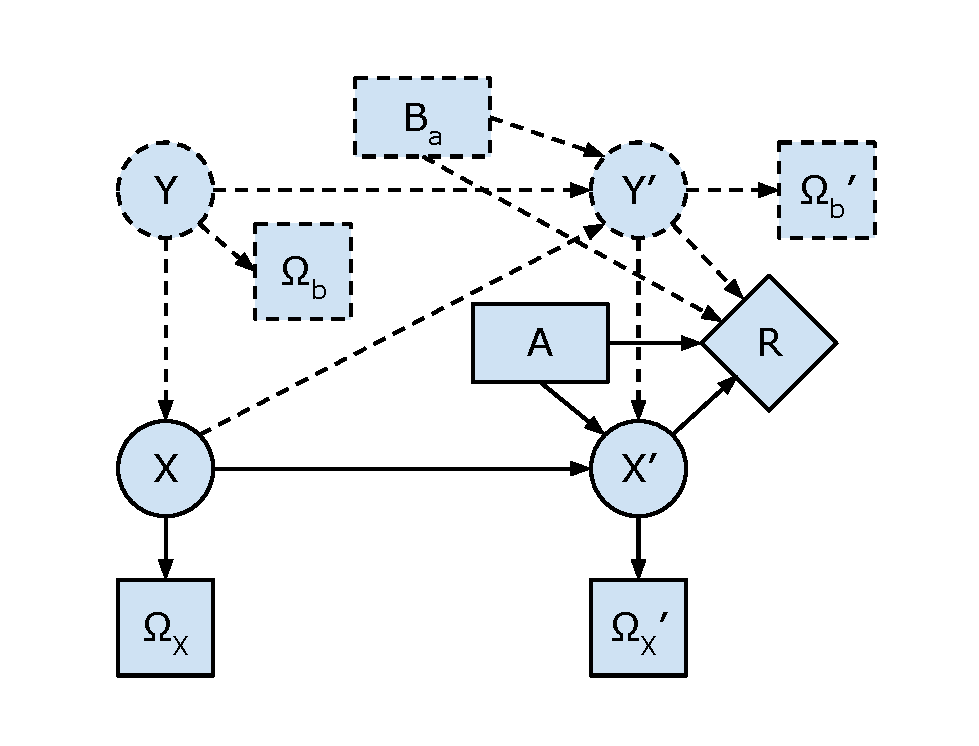
\includegraphics{fig-pomdp.pdf}
\caption{A time slice of a general POMDP (solid lines) and a POMDP augmented with affective states (dotted lines)}
\label{fig:pomdp}
\end{figure}

A partially observable Markov decision process (POMDP) is a general stochastic model that has been extensively studied in operations research and in artificial intelligence \cite{monahan1982state, poupart2011introduction}. Figure~\ref{fig:pomdp} shows a time slice of a general POMDP (solid lines). Capital symbols (e.g. $X$) are used to denote variables or features, small symbols (e.g. $x$) are to denote values of these variables, and boldface symbols (e.g. $\mathbf{X}$) are to denote sets of variable values. Primes are used to denote post-action variables, so $x'$ means the value of the variable $X$ after a single time step. As shown in the figure, a POMDP consists of a finite set $\mathbf{X}$ of states $X$; a finite set $\mathbf{A}$ of actions $A$; a stochastic transition model $Pr : X \times A \to \Delta(\mathbf{X})$, where $Pr(x'|x, a)$ denotes the probability of moving from state $x$ to $x'$ after an action a is taken, and $\Delta(\mathbf{X})$ is a distribution over $\mathbf{X}$, a finite observation set $\mathbf{\Omega\_{X}}$, and a reward assigning function $R(A, X')$. The reward function $R(a, x')$ for each state $x$ denotes the reward received to transit to $x'$ induced by action $a$. A stochastic observation model $Pr : X \to \Delta(\mathbf{\Omega_{X}})$ is used to denote the probability of making observation $\omega$ while the system is in state $x$. Basing on the aforementioned elements, a policy can be developed to map belief states (i.e. distributions over $X$) into choices of actions, such that the expected discounted sum of rewards is (approximately) maximized. POMDPs have been used as models for many human-interactive domains, including human assistance systems \cite{hoey2010automated}.

Figure~\ref{fig:pomdp} (dotted lines) shows a time slice of a general POMDP augmented with affective states. In addition to the basic POMDP elements, affective states $\mathbf{Y}$ are included in the POMDP process. $\mathbf{Y}$ describes the system's beliefs of the user's emotional states. Similarly to $\Omega_{X}$ and $A$, $\Omega_{b}$ denotes observations of user behaviours that gives the system evidence about state $Y$, and $B_{a}$ is the affective meaning of system action that can cause state $Y$ to change. Finally, the reward function $R(A, X', Y')$ is defined over state-action pairs and rewards those states and actions that are beneficial overall to the goals of the system-human interaction. 

\subsection{BayesACT}

ACT models interactions between two persons with a prerequisite that the identities of the two communicators are known to each other. This prerequisite has limited its usefulness in our application, where the user's identity is unpredictable. On the other hand, a Bayesian version of the ACT theory, called BayesACT, was formulated in Hoey et. al.'s work \cite{hoey2013bayesian}. This new model can maintain multiple hypotheses about identities and behaviours simultaneously as a probability distribution, and can make value-directed action choices. By employing BayesACT, machines are able to generate affectively believable interactions with people by learning about their identity, predicting their behaviours, and taking actions that are simultaneously goal-directed and affect-sensitive.

\begin{figure}[p]
\centering
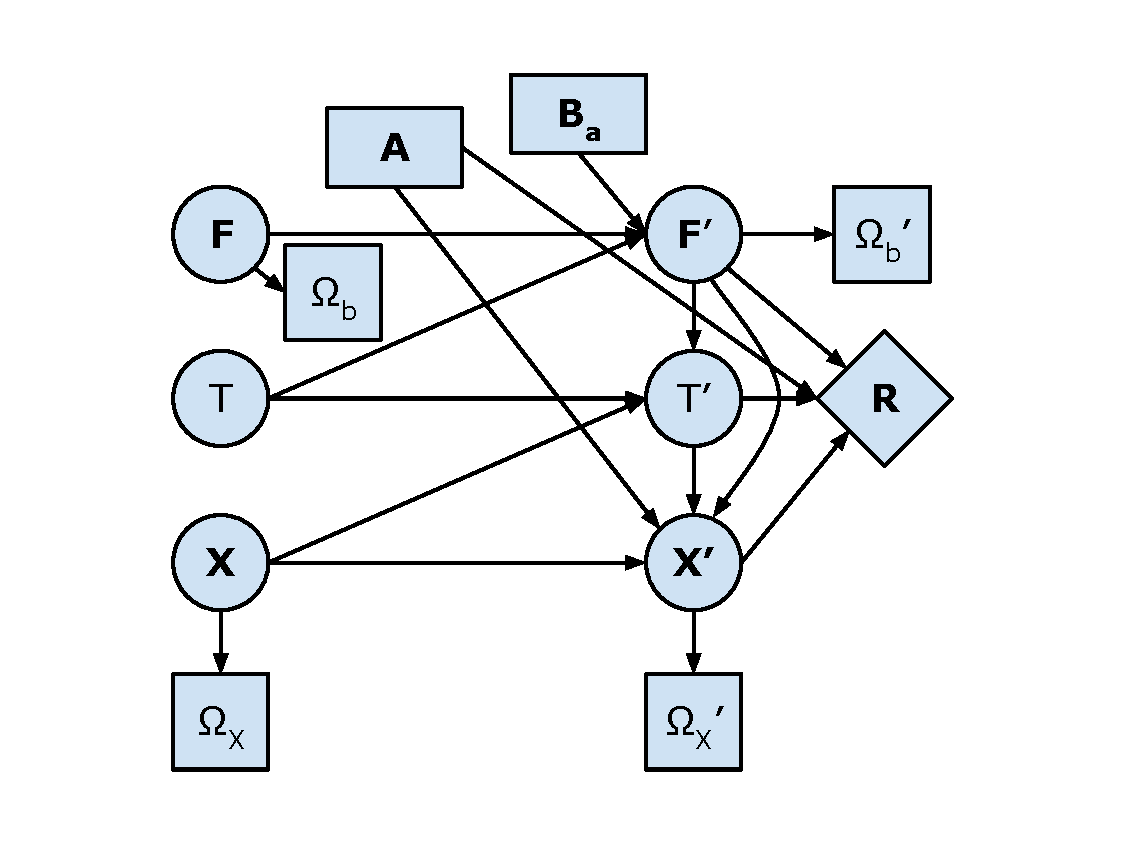
\includegraphics{fig-bayesact.pdf}
\caption{A factored POMDP for Bayesian Affect Control Theory}
\label{fig:bayesact}
\end{figure}

Figure~\ref{fig:bayesact} shows a factored POMDP for the BayesACT. It describes, from the perspective of the agent (although this is symmetric), how the variable state changes based on an interaction between an agent (i.e. a machine) and a client (i.e. a human). In the figure, capital symbols (e.g. $F$, $T$) denote variables or features. Small symbols (e.g. $f$, $t$) denote values of these variables, and boldface symbols (e.g. $\mathbf{B_{a}}$) denote sets of variable values. Primes are used to denote post-action variables, so $x'$ means the values of the variable $X$ after a single time step.

In the figure, $X$ is used to represent everything the system needs to know about the system state, for example, the functional state of the agent and the client. To indicate which party acts at the given time step, $X$ encodes turn-taking messages as well. In BayesACT, Actor-Behaviour-Object grammar (i.e. \textit{Actor Behaves} towards \textit{Object}) is used to describe the simplest social event in the model. $F = \{F_{ij}\}$ denote the set of fundamental sentiments the agent holds, where each feature $F_{ij}, i \in \{a, b, c\}, j \in \{e, p, a\}$ denotes the $j$-th value of the $i$-th interaction object: $a$ (actor), $b$ (behaviour), or $c$ (client). Similarly, $T = \{T_{ij}\}$ is defined and denote the set of transient sentiment the agent holds. Variables $F_{ij}$ and $T_{ij}$ are continuous valued and $F$, $T$ are each vectors in a continuous nine-dimensional space. Note that $F$ and $T$ are encoded as being for agent and client, regardless of who is currently acting in the BayesACT model. The observations $\Omega_{X}$ and $\Omega_{b}$ are anything the system observes in the environment that gives it evidence about the variables $X$ and $F$, such as the actions the agent and the client have taken. The system action $A$ denote the propositional content of a system action (e.g. to instruct the user to perform a behaviour), and $B_{a}$ denote how the message should be expressed (e.g. with a friendly tone). Variable values $\mathbf{B_{a}}$ are three-dimension vectors, i.e. EPA vectors.

%To sum up, the BayesACT model includes states $S = \{F, T, X\}$, observations $\Omega = \{\Omega_{X}, \Omega_{b}}$, and actions A = {A, Ba}. Among the state symbols, Y = {F, T} represents the emotional state of the client, and X represents the functional state of the client. A state S is a probability distribution over the emotional state Y and functional state X of the client. S is updated given the history of actions A and observations . By updating F, the probability distribution of the client's identity Fc is learned. BayesACT can also predict the client's next behaviour and calculate {A, Ba} basing on this prediction given the current belief state of {F, T, X}. The following essential concepts and formulas are defined in BayesACT:

- The de?ection between fundamental sentiments F and transient impressions T, denoted as  (F,T), is defined as a nine-dimensional weighted Euclidean distance between F and T. The distance measure is proposed by the authors of [23] as the logarithm of a probabilistic potential: (f,t)?e-(f-t)T-1(f-t), where  is a general representation of weights. 

- The probability of a post-action fundamental sentiments f' is computed by combining the deflection (f',t') with an "inertial" term that stabilises the fundamentals over time. It gives the probabilistic generalisation of the Affect Control Principle (Definition 1). This can be illustrated by the following formula:
%Pr(f'|f,t,x,ba,)?e-(f',t')-(f',f,ba,x), where t' can be computed from {f', t, x} by empirically derived prediction equations of ACT, and  represents the temporal dynamics of f encoding both the stability of a?ective identities and the predictive dynamics of a?ective behaviours. ? is such that: 1) fb' = ba if the agent is acting, and unconstrained if otherwise; 2) fa' and fc' are likely to be close to fa, fc, respectively.

- Pr(x'|x,f',t',a) is defined to denote how the application progresses given the previous state, the fundamental and transient sentiments, and the (propositional) action of the agent. 

-Pr(b|f) and Pr(x|x) are observation functions for the client behaviour sentiment and system state, respectively. These functions are stochastic in general.

\section{Related Work}
\subsection{Use Assistive Technologies to Help Elders}

According to the United Nation's population report, we are experiencing an aging world. While many elders remain healthy and productive, overall this segment of the population is subject to physical and cognitive impairment at higher rates than younger people. More and more new technologies that incorporate AI methods have been explored to build assistive systems that can help with elder's everyday lives. Pollack \cite{pollack2005intelligent} surveyed such systems, focusing on the ones that support older adults who are grappling with cognitive decline.

Assistive technology can assist older people with cognitive impairment in one or more of the following ways \cite{pollack2005intelligent}: (1) Assurance system (e.g. \cite{hoey2012lacasa}) where the primary goal is to ensure safety and well-being of elders. A caregiver is alerted if the elder is detected not performing well; (2) Compensation systems (e.g. \cite{boger2005decision, peters2014automatic, hoey2010automated}) where the primary goal is to help the elder perform daily activities, i.e. monitoring and giving out prompts when necessary; (3) Assessment systems that aim to assess the elder's cognitive status. While it is obvious that the ability to observe, recognize and reason about the elder's performance of daily activities is essential for assurance systems, this ability is equally important for both assistive systems and assessment systems: the more accurately an assistive system can recognize activities and estimate a user's current state and needs, the more useful assistance it can provide; the better an assessment system can recognize daily activities and reason about how and when an user perform these daily activities, the better assessment of the user's cognitive state it can provide.

Activity recognition is currently a very active research topic. Work has been done to use sensors to monitor the execution status of particular types of activities, such as handwashing \cite{hoey2010automated}, meal preparation \cite{philipose2004inferring}, and movements around town \cite{hoey2012lacasa}. In general, Bayesian networks are the principal technology used for performing activity recognition. A typical approach is taken in the PROACT system \cite{philipose2004inferring}, which employs a dynamic Bayesian network that represents daily activities such as making tea, washing, brushing teeth, and so on. In their approach, radio frequency identification (RFID) tags are attached to household objects and the user of PROACT wears a specially designed glove that includes an RFID reader. Since special gloves are required in the PROACT system, this approach is somewhat inconvenient for users. Another assistive system example, the COACH system \cite{boger2005decision, hoey2010automated}, used a Bayesian network. In the COACH system, images are grabbed by a camera mounted above the sink, and fed into a hand and towel tracker. The tracker then processes these images and reports the positions of the hands and towel to a belief monitor that uses a POMDP framework and a Bayesian network to estimate where in the task the user is currently: what they have managed to do so far, what their internal mental state is, etc. The belief of the user's state is passed to a policy processor, where belief states are mapped into actions: based on the belief states, the system may play out audio-visual prompts, call for human assistance, or do nothing. The COACH system is more user-friendly than the PROACT system in the sense that it doesn't require the user to wear any specific devices.

While accuracy is a desirable feature for assistive systems, it is equally important for these systems, especially the ones that are designed to monitor older people performing daily activities and give out helpful prompts when necessary, to have high quality human-computer interaction (HCI). In fact, as more and more intelligent objects (physical robots, programs, etc) are being developed, more and more research has been conducted in the field of HCI. Viewing HCIs as a social activity, Suchman reviewed how agents are currently configured and stated her view of how they might be reconfigured in her 2007 book \cite{suchman2007human}. As Suchman pointed out, the planning model was at that time (and probably still is) the dominant model for intelligent machines and rational action; however, the situated part has been neglected in such models.

Being a large subset of intelligent objects, systems that can provide guidance to humans are built to reason about observations towards certain objectives and act based on their reasoning. The effectiveness of these assistive systems not only relies on the accuracy of user-behaviour recognition and rational planning, but also depends on how well the user understands the instructions these systems give out. To achieve the goal of communicating purpose to users more effectively, actions of the system are required to encode more local situational factors, such as awarenesses and emotional states of the user at that time. The COACH system \cite{hoey2010automated} took a step towards this direction by including variables that describe the user?s state, such as awareness, responsiveness and overall dementia level. However, the user's emotional state was not considered by the system when giving out behaviour suggestions.

\subsection{Including Emotional Intelligence in HCIs}

It has been widely agreed that the essence of emotional intelligence should be included in next generation of HCIs. Studies have shown that being capable of detecting and responding appropriately to its users' affective feedback can make a HCI system act more naturally and effectively. The topic of using emotional intelligence in HCI is mainly concerned with four main aspects: (1) \textit{recognition of affective states}, example approaches include vision-based, acoustic-based, and modality approaches \cite{pantic2003toward, zeng2009survey}; (2) \textit{generation of affectively modulated signals}, such as speech, facial and bodily expressions \cite{cassell2000embodied, niewiadomski2013computational}; (3) \textit{psychological study of human emotions}, including affective interactions and adaptation \cite{scholl2013socio}; (4) \textit{computationally modelling affective human-computer interactions} \cite{hoey2013bayesian, pynadath2005psychsim, el2000flame, conati2009empirically}. While research covering one or more of these topics have been conducted, few real-world applications that combine all of the four pieces together has been implemented. This thesis takes a look at each of these aspects and designs and builds an assistive system that integrates all four pieces together and harnesses the benefits of including emotional intelligence in HCI.

\subsubsection{Affective States Recognition}

A large body of psychological studies have been conducted on examining how factors influence human emotions and how can these emotions be measured. While there is no single gold-standard method for measurement of one's emotions, it is widely agreed that emotions consist of variably interrelated changes in activity across a set of five components \cite{scherer2005emotions}: (1) appraisals of event, (2) psychophysiological changes (bodily sensation), (3) motor expressions (face, voice, gestures), (4) action tendencies, and (5) subjective experiences (feelings). Table~\ref{table:emotion-factors}, borrowed from \cite{scherer2005emotions}, gives some examples of values for these factors.

\begin{table}
\centering
\caption{Five factors that can cause emotional changes (from \cite{scherer2005emotions})}
\label{table:emotion-factors}
\begin{tabular}{| p{4.4cm} | p{10.8cm} |}
\hline
\multirow{7}{4.4cm}{Appraisals of eliciting event (E)} & How suddenly and abruptly did E occur? \\
& How familiar was the person with E? \\
& How pleasant/unpleasant is E in general, independently of the current situation? \\
& How important/relevant is E to the person's current goals or needs? \\ 
& ... \\
\hline
\multirow{5}{4.4cm}{Physiological Symptoms} & Feeling cold shivers (neck, chest), Weak limbs, Getting pale \\
& Lump in throat, Stomach troubles \\
& Heart beat slowing down/getting faster \\
& Muscles relaxing/tensing, restful/trembling (whole body) \\
& ... \\
\hline
\multirow{5}{4.4cm}{Motor Expressions} & Smiling, Frown, Tears \\
& Mouth opening, closing, tensing \\
& Eyes closing, opening \\
& Voice volume increasing \\
& ... \\
\hline
\multirow{5}{4.4cm}{Action Tendency} & Moving attention towards/away from E \\
& Information search \\
& Attention self-centered/directed towards others \\
& Physically moving towards/away from E \\
& ... \\
\hline
\multirow{2}{4.4cm}{Subjective Experiences} & Intensity, Duration, Valence, Arousal, Tension \\
& ... \\
\hline
\end{tabular}
\end{table}

With all these indicators of emotional changes, in the context of automatically recognizing affective states using computers, approaches analysing both verbal and nonverbal behaviours have been conducted.

Studies concerned with ``verbal behaviours'', such as words selected in an interaction, is probably one of the most mature ones in the domain of sentiment analysis. Several dictionaries mapping words into affective meanings have been constructed by human raters in survey-based studies and have been released for public accessibility online\footnote{See \url{http://www.indiana.edu/~socpsy/ACT/data.html} for a list of the dictionaries.}. Several computer programs have been implemented based on these dictionaries to describe and predict people's emotional states and behaviours in given situations. Among all these programs, INTERACT\footnote{Accessible via \url{http://www.indiana.edu/~socpsy/ACT/interact.htm}.}, is an interesting one to note.

One the other hand, studies from the point of view of ``non-verbal behaviours'' attempt to extract human emotions from their facial, bodily, vocal expressions, and other non-verbal behaviours during an interaction. Studies in psychology have shown that non-verbal behaviours is an important channel for expressing emotions as well \cite{schroder2013culture}, and that in real-life scenarios, selection of words does not necessarily reflect the actor's affective states. Furthermore, recognizing words used in real-life conversations is likely to be very difficult, especially when the communicating parties are feeling intensive emotions. Realizing the importance and advantages of non-verbal behaviour analysis, more and more work in this domain has emerged in recent years. While humans can detect and interpret interactive signals of their communicators with little or no effort, it is much more difficult to design and develop an automated system that accomplishes the same tasks. In the following paragraphs, we survey several examples of tackling the problems of machine detection and interpretation of human affective states from non-verbal behaviours, focusing on facial expression analysis and body movement analysis. Readers are recommended to refer to Pantic's work \cite{pantic2003toward} and Zeng's work \cite{zeng2009survey} for a more comprehensive review of previous work.

Vision-based and acoustic-based are two most common approaches in the domain of automatic detection of emotions from non-verbal behaviours. Recognizing the important role facial expression plays in delivering affective messages, a fairly large amount of vision-based methods have been applied to detect emotion from facial expressions. A typical first step of this detection is to get an objective description of facial expressions, leaving the judgement of emotional message underlying these signals to a higher-level of decision making. The Facial Action Coding System (FACS) \cite{ekm02}, for example, is one of the most comprehensive and widely used sign judgement systems. In this anatomically-based system, visible effects of facial muscle activations are described by ``action units'' (AUs), after which high-level decision-making processes aiming to learn the underlying affective meanings of facial expressions are applied on the AU representations. One most desirable feature of using AUs and AU descriptors is its ability of representing the thousands of anatomically possible facial expressions that humans can perform, independently of what high-level interpretations these facial expressions may imply. Bartlett's work \cite{bartlett2005recognizing} is an example work that has taken this approach. However, building automatic AU detectors is not as easy as one might think. One difficulty in designing such auto-detectors comes from the differences, such as face shape, texture and behaviours, between individuals. This inter-personal difference in facial structures would affect the performance of automatic AU detectors, and thus indirectly affect the performance of a generic classifier on top of the AU detectors applying to unseen persons. A recent work \cite{chu2013selective}, Selective Transfer Machine\footnote{Program basing on this method is accessible via \url{http://www.humansensing.cs.cmu.edu/intraface/}.} (STM), attempted to tackle this problem by personalizing a generic classifier in an unsupervised manner. Another problem researchers face when designing automatic AU detectors is that changes in pose, scale, illumination, input clearance, etc, can all cause different levels of visible effects changes of the same facial movements. To tackle this problem, as complement to the old databases which contain only front-view facial-movement recordings, databases consisting of profile-view \cite{pantic2005web} and even 3-D recordings \cite{yin20063d} of facial expressions have been built up. In addition, realizing that ``deliberate behavior differs in visual appearance, audio profile and timing from spontaneously occurring behaviours'' \cite{zeng2009survey}, databases consisting of spontaneous facial expressions (including interview recordings to collect spontaneously expressions) have been built as well.

Studies have shown that bodily expressions encode affective messages as well \cite{schroder2013culture, coulson2004attributing}. In fact, in situations where accuracy of analysis on facial expression might be affected, for example, situations where perception is from a distance, or situations where affective states can be conveyed through movements more easily, better results are likely to be achieved by including bodily expressions in affect analysis. However, while facial expression analysis has been receiving much attention in the context of emotion recognition, much less research on automatic recognition of bodily expressions has been done. Two recent surveys \cite{kleinsmith2013affective, karg2013body} reviewed work on recognizing affect from bodily expressions using computational models, compared this kind of approach with that from the point of view of facial expression analysis, and discussed challenges researchers face in this field, such as the challenges in data collecting, labeling, modeling, the challenges in setting up benchmarks, and the ones in dealing with inter-individual and inter-cultural differences.

A typical process of automatic affect recognition of bodily expressions includes the following steps \cite{karg2013body}:
\begin{enumerate}
\item collecting motion trajectories from sensor data,
\item segmenting data collected based on time windows or movement primitives,
\item describing segmented data using the selected feature set,
\item mapping the representation from last step to affective states.
\end{enumerate}
Step 1 and 2 address human movement analysis in general (i.e. not limited to affect recognition). With appropriate temporal segmentation being a common challenge faced by researchers from many fields (including those from facial expression analysis as well), most current studies use pre-segmented data. As for step 3, the following three approaches, or combination of them, are generally used for constructing feature spaces \cite{karg2013body}: (1) Features describing human movement are hand-chosen and reduced by dimensionality reduction when necessary (e.g. \cite{nicolaou2011continuous}). This approach is most suitable in situations where sensor data cannot easily be related to a kinematic or shape-based model of human motions, for example, when sensor data is collected from a pressure sensor integrated in a seat (e.g. \cite{d2009automatic}). The disadvantage of this approach is that it is not grounded in psychological theories. (2) Features are selected based on findings from perceptual studies in psychology (\cite{karg2010recognition}). (3) Features are defined as high-level descriptors in a movement notation system (e.g. \cite{castellano2007recognising}). Similar to facial expression analysis, a good movement notation system is beneficial to bodily expression recognition as well. However, despite the fact that several movement notation systems have been proposed (e.g. \cite{birdwhistell2011kinesics}), we still lack a widely-recognized notation system that can help map between movements and affective states quantitatively. Again, these three approaches are not mutually exclusive; on the contrary, they are usually combined together. It is interesting to note that across all the approaches, movement speed is selected as a feature in most studies. A rather comprehensive review on features that have been selected in previous works has been given in Kleinsmith's survey \cite{kleinsmith2013affective}. 
Step 4 aims at mapping representations of features to affective states. Results in previous studies \cite{beck2010interpretation} have shown that velocity and expansiveness correlate with arousal, and that the basic posture relates to the expressed evaluation of valence, with a contracted posture for low valence and an open posture for high valence. In this step, classifiers are usually trained and/or regression techniques are usually applied. One can find an overview of machine learning methods that have been applied in previous studies in Klensmith's survey \cite{kleinsmith2013affective}.

Aside from vision-based approaches, acoustic-based approaches have also been taken for affect recognition. Popular acoustic features used in existing approaches include prosodic features (e.g. pitch-related features, energy-related features and speech rate) and spectral features (e.g. MFCC and cepstral features). Among all these features, pitch and energy have been reported to contribute the most to the speaker's affective states in studies on ``artificial'' datasets (e.g. \cite{kwon2003emotion}). However, as indicated by Batliner et al. \cite{batliner2003find}: ``The closer we get to a realistic scenario, the less reliable is prosody as an indicator of the speaker's emotional state''. Some work \cite{lee2005toward} included words spoken in emotion detection as well and improvement was indicated. However, including words spoken as a feature in practical automatic affect detection systems might be infeasible or even unnecessary. First, whether current automatic speech detection can reliably recognize words spoken in emotional speeches is unknown \cite{athanaselis2005asr}. Second, relationships between words chosen and the speaker's affective states have been reported to be rather unreliable \cite{ambady1992thin}. Third, the association between linguistic content and emotion is language dependent, which certainly affects the performance of an affect detector applied to a language different from the one it was trained upon.

As discussed in Zeng's survey \cite{zeng2009survey}, open questions in affect recognition also include: utilizing contextual information, such as environment, observed subject, or the current task, in the process of affect recognition; appropriately segmenting data collected for analysis; constructing a dataset and setting up a benchmark that is shared by researchers within the field.

\subsubsection{Affective Signals Generation}

Generation of affectively modulated signals, which falls into the second aspect of including emotional intelligence in HCI, is to some extent the reverse of affect recognition. A typical process of such generation includes following steps \cite{karg2013body}:
\begin{enumerate}
\item deciding affective state to be encoded,
\item selecting movement type (e.g. facial expressions or bodily movements), based on the affective state decided in last step, or the functional task to accomplish,
\item modulating movement affectively, which means to add affective expressiveness to functional or abstract movements,
\item generating trajectories (and/ or carrying out motor commands for robots).
\end{enumerate}
Depending on application scenarios, different movement types can be chosen and different movement modulation techniques can be used. 

Adding affective signals to movements is believed to be beneficial to enhancing the believability of a virtual agent or robot \cite{lasseter1987principles}. Animators at Walt Disney Studios have proposed a set of 12 design principles to create believable characters, among which four are associated with the expression of affective states \cite{lasseter1987principles, kerlow2004art}. Aside from the studies and experiences in the animation industry, research in developing well-performed embodied conversational agents (ECAs) has examined the importance of techniques in affective signal generation as well. ECAs are virtual entities with human-like communicative capabilities \cite{cassell2000embodied, niewiadomski2013computational}. ECAs communicate through verbal and nonverbal communication channels such as facial expressions, hand and arm movements, body posture, and prosody. Models to create behaviours based on emotions described by both categorical labels and dimensional representations have been proposed. To enrich the emotional behaviours of a virtual agent, some of the models that rely on discrete facial expressions used fuzzy methods (e.g. \cite{bui2004creating}). More commonly, models based on a dimensional approach are used because they allow the creation of a variety of expressions with subtle differences for related emotional states. Boukricha et al. \cite{boukricha2009pleasure} proposed a FACS \cite{ekm02} based model to generate facial expressions from emotions described by three-dimensional Potency-Activity-Dominance (PAD) vectors. In their approach, randomly generated facial expressions composed of several action units as defined with FACS were evaluated in term of PAD values in an empirical study. The rated expressions were placed in the dimensional space, where Dominance takes one of two discrete values (high/low dominance), while pleasure and arousal values are mapped into a continuous space. With the help of multivariate regressions, the authors are able to map from PAD values to facial expressions. While most research on models of emotional displays focus on facial expressions, interest in multimodal expression of emotions in ECA have recently emerged. Findings in psychological studies have shown that emotions are expressed through a set or a sequence of different nonverbal behaviours, rather than a static facial expression. Niewiadomski et al. \cite{niewiadomski2013computational} surveyed several models that have introduced multimodality and sequentiality into generation of affective signals.

Dynamic generation of affective movements requires the processing of multivariate contextual information and much computational resources. Thus, in our prototypical handwashing system, based on the affective signals needed, the system selects a most appropriate affectively modulated prompt from a set of pre-generated and rated prompts. The set of pre-generated prompts were created and evaluated in Malhotra's work \cite{malhotra2014}.  Malhotra designed 30 emotionally aligned prompts that could be used by a cognitive assistive system in a handwashing scenario. Three dimensional vectors in EPA space were used to represent the emotional interpretations of the prompts. The prompts covered all of the five situations where the system needs to suggest the user to ``turn on the water'', ``use some soap'', ``rinse your hands'', ``turn off the water'' and ``use the towel''. For each of these propositional actions, Malhotra designed the prompts to cover five cases where the same message was expressed with emotional impressions of ``kind, powerful, active'', ``kind, powerless, inactive'', ``mean, powerful, active'', ``mean, powerless, inactive'', and ``kind, powerless, active''. The two screenshots captured from Malhotra's prompts in figure~\ref{fig:} \textcolor{red}{add figure} shows how the prompts look like. An online survey was conducted in which participants were asked to watch the 30 video prompts and rate them based on Evaluation, Potency, and Activity dimensions (on a discrete scale of $-4$ to $+4$ with increments of 1 for a total of 9 options). The questions were presented in random orders and participants were able to exit the survey at anytime. There were a total of 27 respondents (16 male/9 female with 18 nationals and 9 internationals) who answered more than 90\% of the questions. Analysis showed that participants' answers were consistent with each other. The mean of all valid ratings of a prompt was then computed as the final EPA vector for that prompt. With the correspondence between EPA values, instructional content, and the prompts generated by Malhotra, we are able to select at a given timestep a most appropriate prompt based on the required affective signals and instructional contents.

\subsubsection{Psychological Study and Computational Models of Emotional Interactions}

There exists a large body of work in psychology and sociology that studies human emotions and their roles in interactions. In these studies, emotions are usually represented as categorical labels, or dimensional values. Models, such as ACT \cite{robinson2006affect}, describing how people perceive emotions and how their interactions are regulated by these emotions have been proposed. Section~\ref{sec:concepts} Basic Concepts should give readers a conceptual overview of the studies of human emotions; a more comprehensive review of this area is beyond the scope of this thesis.

Basing on findings in studies of human emotions, significant work in affective computing that uses probabilistic reasoning to build intelligent interactive systems have emerged. Psychsim \cite{pynadath2005psychsim} is an example of such interactive agents. In Psychsim, a POMDP model of psychological consistency theories was employed to estimate the relative value of actions. Various appraisal dimensions and a variety of influence factors such as consistency, self interest and ``bias'' was used. However, since the dimensions and influence factors were defined in an application-specific manner, it is not clear if they would generalise to other applications. A second example of such systems is FLAME \cite{el2000flame}. FLAME combined fuzzy logic with reinforcement learning to achieve adaptivity. Emotional states and actions in FLAME were generated following application-dependent appraisal rules based on the OCC model \cite{ortony1990cognitive} and a set of ad-hoc rules, respectively. Conati and Maclaren's work \cite{conati2009empirically}, which used a decision theoretic model and relied on sets of labelled emotions and rules from appraisal theories, is another example of an affectively intelligent interactive system. However, coming along with the advantage of easing interpretability and computability, and allowing for the encoding of detailed prior knowledge into applications, are the difficulties of generalization rule-based approaches have to face.

Different from rule-based systems, BayesACT \cite{hoey2013bayesian} used a more general set of appraisal dimensions and describes identities and behaviours by values of these dimensions, regardless of their high-level interpretations. By operating completely in a dimensional space, BayesACT is able ``to surmount computational issues, to assure scalability (the state space size only grows with the amount of state necessary to represent the application, not with the number of emotion labels), and to explicitly encode prior knowledge obtained empirically through a well-defined methodology'' \cite{hoey2013bayesian}. A python program (denoted as BayesAct), including both a tutoring-system version and a simple handwashing-assistant version, based on the BayesACT model was implemented for simulation and test purposes. Some parameters that need to be set when using this reasoning engine is described in Table~\ref{table:bayesact-param}; for a more complete list of the parameters, see paper \cite{hoey2013bayesian}. Despite the fact that the BayesACT model is easy to generalize for different applications, and thus can potentially be used as an emotional ``plug-in'' for systems that interact with humans, converters that map between actions (from both human users and the system) and dimensional values are still required for it to work in a real-world scenario. In other words, the BayesACT model did not tackle the problems of affect recognition and generation.

\begin{table}
\centering
\caption{Some of the parameters that need to be set when using BayesAct}
\label{table:bayesact-param}
\begin{tabular}{| l | l | p{9.4cm} |}
\hline
param & default value & meaning \\ \hline
$\beta_{a}^{0}$ & $0.01$ & initial identity variance for agent (larger means agent is more uncertain of its own identity) \\ \hline
$\beta_{c}^{0}$ & $0.01$ & initial identity variance for client (larger means agent is more uncertain of the client's identity) \\ \hline
$\gamma$ & $(1.0, 1.0, 1.0)$ & model noise variance of the E, P, and A values of user behaviours (larger means agent is more uncertain of the input) \\ \hline
$N$ & $300$ & number of samples used in the computation \\ \hline
$f\_a^{0}$ & not mentioned in \cite{hoey2013bayesian} & initial identity of agent \\ \hline
$f\_c^{0}$ & not mentioned in \cite{hoey2013bayesian} & initial identity of agent \\ \hline
\end{tabular}
\end{table}

\subsection{Hands Recognition Approaches}

Noting the importance of accurately recognizing and tracking the user's hands in a hand-washing system, several typical hand tracking approaches are reviewed in the following paragraphs; note that formal analyses of and comparisons between these methods is beyond the scope of this thesis.

One approach of recognizing hands and other objects based on skin-color \cite{mihailidis2004use}. In this approach, statistics-based color segmentation models and background subtraction were combined to identify objects, such as the user's hands and the towel, within the field of view. This approach is independent of time and thus is only able to recognize objects (rather than to track them). Another disadvantage of this method is that it is prone to noise, in the sense that skin colors of an object can change due to lighting-condition changes in the environment. A vision-based agent, which utilized this approach to recognize the user's hands and the towel, has been developed to assist persons with dementia during handwashing \cite{boger2005decision}. The locations of the user's hands and the towel are extracted by the agent for each frame, and the locations of other objects (e.g. the soap) are predefined in the approach. The user's hand behaviours are then detected by comparing the hands' locations with other objects' locations, and are used to update the beliefs of where the user is at during the handwashing process. 

Another method to track hand locations is to use flocks of features \cite{hoey2006tracking}. A flock is a loose collection of features, or members. The features are characteristics of the local appearance of the object that is to be tracked. An approximate Bayesian sequential tracking method that uses flocks of color specks was used in a previous work of Hoey et. al. \cite{hoey2006tracking}. To allow for long-term tracking of multiple objects, the authors also used a combination of three mixed-state particle filters \cite{isard1998mixed} with data-driven proposals \cite{okuma2004boosted} and simple interactions to enable reinitialization after a track is lost. The method is robust to partial occlusions, distractors and shape changes. It is also able to consistently track objects over long sequences; as opposed to the previous ones which are independent of time.

Different from the above approaches, Czarnuch and Mihailidis utilized the depth information of images to track human bodies \cite{czarnuch2014}. A C program was developed and tested to track the user's body parts (such as head and hands) from an overhead perspective. The program has no prerequisites on environmental conditions or physical settings of the system, other than that images should be grabbed with depth information from an overhead perspective, which is easy to satisfy by mounting a RGBD camera above the sink area. The tracker was trained using partially labeled, unbalanced data, and has been shown by the authors in their paper that it is able to recognize and track the user's hands. The tracker is also configurable and re-trainable. One could recollect data and retrain the tracker if the tracker is to run in an environment different from the one which it was trained in. All these desirable features of the tracker make it a good candidate to design and develop our hand-washing system upon. More approaches on tracking human body parts using depth information of images can be found in Czarnuch and Mihailidis's paper \cite{czarnuch2014}, and Shotton et. al.'s work \cite{shotton2013real}.
\chapter{System Design}
\label{chap:design}

Our goal is to design an extensible system that can assist people with dementia during a hand-washing process by assessing their states and provide instructions accordingly. The system should combine affect recognition of behaviours, affective reasoning during interactions, and affective signals generation with AI techniques. This chapter illustrates how our system is designed as an integration of independent components. 

People with certain types of cognitive disabilities have trouble in accomplishing daily tasks. For example, persons with dementia tend to forget where they are in a handwashing task, and without a caregiver's reminder, they might not be able to proceed. However, the need of human assistance in everyday tasks can cause the persons with dementia to feel unconfident and depressed. The frustrating caring jobs could also add a burden to families.

An assistive handwashing system is a cognitive intelligent system that can monitor user's behaviours and give proper prompts at certain times. Basically, the system observes the outside world and analyzes the observations over time. At each time step, the system updates its belief states about where the user is at in the handwashing task, and if needed, gives out proper prompts based on these belief states. One limitation of previously-built handwashing systems is that they did not consider users' emotional state changes during the interactions. In other words, the previous systems work functionally, but not emotionally. This defect could limit the effectiveness of the systems when expressing their instructions to human users. The handwashing system we design is able to compute both the user's functional states (i.e. where the user is at during the handwashing process) and emotional states (i.e. the user's identities and emotional states at each time step). The prompts it gives out are produced based on both of the above two states. 

\section{Overview}

\begin{figure}[htp]
\centering
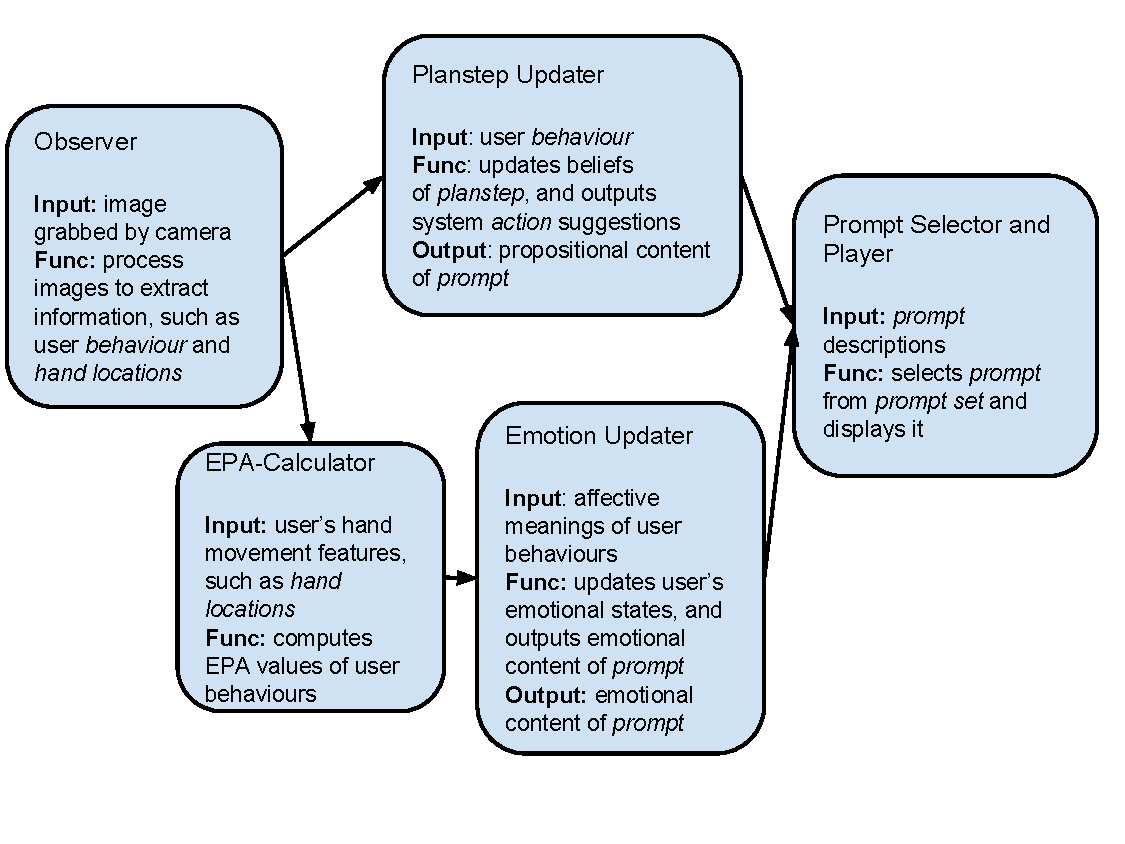
\includegraphics[trim = 0mm 15mm 2mm 5mm, clip, width=0.9\linewidth]{fig/fig-components.pdf}
\caption{Functionality analysis on the system}
\label{fig:components}
\end{figure}

Figure~\ref{fig:components} describes the essential components of the hand-washing system based on a functionality analysis on the system. It shows also the data flow between components in the hand-washing system. The user's movements are observed and parsed in the \textbf{Observer} to extract information, such as user behaviours (e.g. ``turning on water'') and hand locations (i.e. the coordinates of the user's hands). User behaviours are then fed into the \textbf{Planstep Updater}, where beliefs (probability distributions) of where the user is at in the hand-washing process is updated and contents of instructions guiding the user to proceed is decided. On the other hand, hand movement features (such as hand locations) are fed into the \textbf{EPA-Calculator}, where emotion interpretations of the user's behaviours are computed. The \textbf{Emotion Updater} updates the beliefs of the user's emotional state basing on emotional interpretations of user behaviours, and produces the emotional content of the desired system action. Finally, the \textbf{Prompt Selector and Player} of the system selects/generates and displays proper prompts basing on the descriptions. 

In the figure and our descriptions, planstep is used to denote the user's functional state and emotion is used to denote the user's emotional state. Prompt, which is an instructional message displayed by the system to the user, is used interchangeably with system action in our descriptions. The rest of this section analyzes the input, output, functionality and design difficulties of these components. How exactly each component is designed in our approach is explained. For easier description, ``the \textbf{Output Part}'' is used alternatively with ``Prompt Selector and Player'' to refer to the same component.

\section{The Planstep and Emotion Updaters}
\label{sec:design-updater}
\subsection{The Planstep Updater}

Planstep denotes the functional state of a user (i.e. how much has he/she accomplished) during the handwashing task. A set of subtasks of handwashing are defined, and each planstep is a combination of the completeness of these subtasks. For each timestep, the system checks if particular behaviours have been performed and updates planstep beliefs if particular subtasks are accomplished. A general definition of subtasks involved in a handwashing process uses three indicators: whether the water is on (on/off), the soap is on user's hand (dirty/soapy/clean), and the user's hands are wet (dry/wet). The corresponding planstep update diagram of this definition is shown in Figure~\ref{fig:planstep}.

\begin{figure}[htp]
\centering
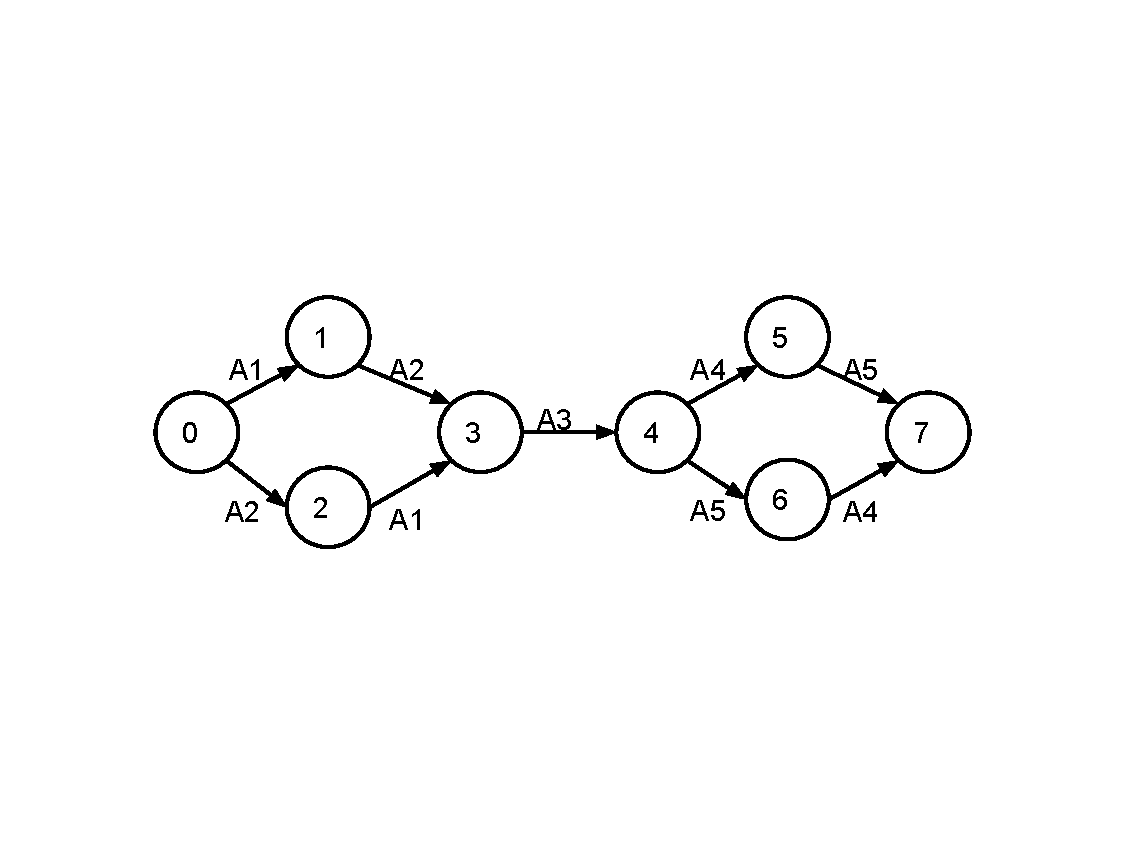
\includegraphics[trim = 20mm 50mm 20mm 50mm, clip, width=0.8\textwidth]{fig/fig-planstep.pdf}
\caption{A planstep update diagram}
\vspace*{2mm}
\parbox{0.85\linewidth}{Integers 0 to 7 denote the eight plansteps this subtask partition defines, which are (0) ``off/dirty/dry'', (1) ``on/dirty/dry'', (2) ``off/soapy/dry'', (3) ``on/soapy/dry'', (4) ``on/clean/wet'', (5) ``off/clean/wet'', (6) ``on/clean/dry'', (7) ``off/clean/dry'', respectively. A1 to A5 represent five behaviours completing the subtasks. A1 to A5 are ``turn on water'', ``put on soap'', ``rinse hands'', ``turn off water'', and ``use towel'', respectively.}
\label{fig:planstep}
\end{figure}

Estimating if a subtask has been accomplished in the handwashing process is the most essential part in the planstep update. This can be broken down into two subproblems: (1) to check if an user behaviour has been performed, which is solved in the Observer; (2) to decide if a subtask has been accomplished accordingly.

Usually, sensors are put around the sink area to collect supportive evidence on recognizing user behaviours. One typical approach is vision-based (e.g. \cite{hoey2006tracking, mihailidis2004use, czarnuch2014}): a camera is mounted above the sink to capture images of the area. For each video frame, by analyzing on the captured images, hands are tracked and their coordinates are obtained. By comparing the positions of the user's hands with the predefined ones of objects (such as soap, towel, sink and water), a system is able to check if the user's hands are within the neighbourhood of a certain object. If a certain area is detected, then the corresponding user behaviour is implied. For example, if the user's hands are detected to be in the neighbourhood of the soap, then he/she is believed to be putting on some soap on his/her hands. 

Note that even if the hand locations are extracted without errors (which in reality is impossible), this location-based approach still can not claim to have 100\% accuracy in detecting user behaviours. This is because having put one's hand in a particular position does not necessarily imply that the person is performing a certain behaviour. For example, the user can simultaneously put his hand on the tap while doing nothing, where a behaviour of ``turning on water'' or ``turning off water'' would be false positively detected by this approach. Adding more sensors (such as pressure sensors for detecting waterflow) might increase the accuracy of user behaviour detection; however, too many sensors is undesirable in our system design. Similarly, due to the subjective nature of the problem, having performed a behaviour does not necessarily imply the completeness of a subtask. For example, even though the behaviour of ``using the towel'' is detected, the dryness of the user's hands is still not predictable without further information. 

Given the partially observable nature of user behaviours and the non-deterministic relationship between a user performing a behaviour and a user accomplishing a subtask, the POMDP model is used to design the Planstep Updater. To model the observation noise and the uncertainty between user behaviours taken and subtask completeness, a probability distribution is associated with each observation and possible behaviour. The probability distribution associated with observations gives the probability that one user behaviour is detected while another user behaviour is actually being performed. The probability distribution associated with behaviours, on the other hand, gives the probability that a subtask has been completed by the user when a certain behaviour is performed. With these two probability distributions, the Planstep Updater is able to update planstep beliefs based on user behaviour observations. Given the planstep of a user, the functional content of the system prompts is then decided based on a policy.

\subsection{The Emotion Updater}

The Emotion Updater in our approach is designed based on the BayesACT model. Three-dimensional vectors that represent \textit{evaluation}, \textit{potency}, and \textit{activity} respectively (i.e. EPA vectors) are chosen to describe affective meanings in our work. Basic concepts of both of BayesACT and ACT are introduced in Section~\ref{sec:concepts} of this thesis. As explained there, ACT can serve as a general psychological principle of micro-regulation of interpersonal interactions and BayesACT is able to learn the identities of users from their behaviours.

According to ACT, large deflections between the immediate impressions that the system prompts have on the user and the user's fundamental sentiments of him/herself and the hand-washing system would cause the user's attention to shift away from the premium communication objectives (i.e. to have his/her hands washed). Thus, it is important for the system to act in a way that is aligned with the user's emotional states. For example, if the user thinks of himself as the ``boss'' in their interaction, a more polite suggestion rather than an order should be given to achieve effective communication. Unfortunately, diseases can cause identity shifts \cite{lively2011identity}, and the identity of a person with dementia is not obvious at all \cite{orona1990temporality, rose2004memory}. Therefore, the user's identity should be learned from his/her behaviours. This thesis designs the Emotion Updater based on the BayesACT model. It represents the identity belief of the user as a probability distribution and updates it using observation functions, where the observations are emotional interpretations (i.e. EPA values) of user behaviours. The Emotion Updater is able to learn the user's identity in theory and in simulation, but not yet evaluated in practice. This thesis only briefly addresses this learning of the identity in the experimental results. 

\subsection{As One Single Reasoning Engine}
\label{subsec:design-singleengine}

The two updaters together decide the functionalities of the Observer and the two together form the functionality center of the hand-washing system. Logically, they both update belief states of the system at each timestep, and compute prompt descriptions based on the beliefs. From an engineering perspective, the two can be combined and developed as a single reasoning engine. In our approach, the two updaters are implemented on the basis of the existing BayesAct framework (implemented in \cite{hoey2013bayesian}). Figure~\ref{fig:updater} shows how this thesis designs the Planstep and Emotion Updater as a single reasoning engine based on the BayesAct framework. Some parameters that need to be set when using this engine are described in Table~\ref{table:bayesact-param}.

\begin{figure}[htp]
\centering
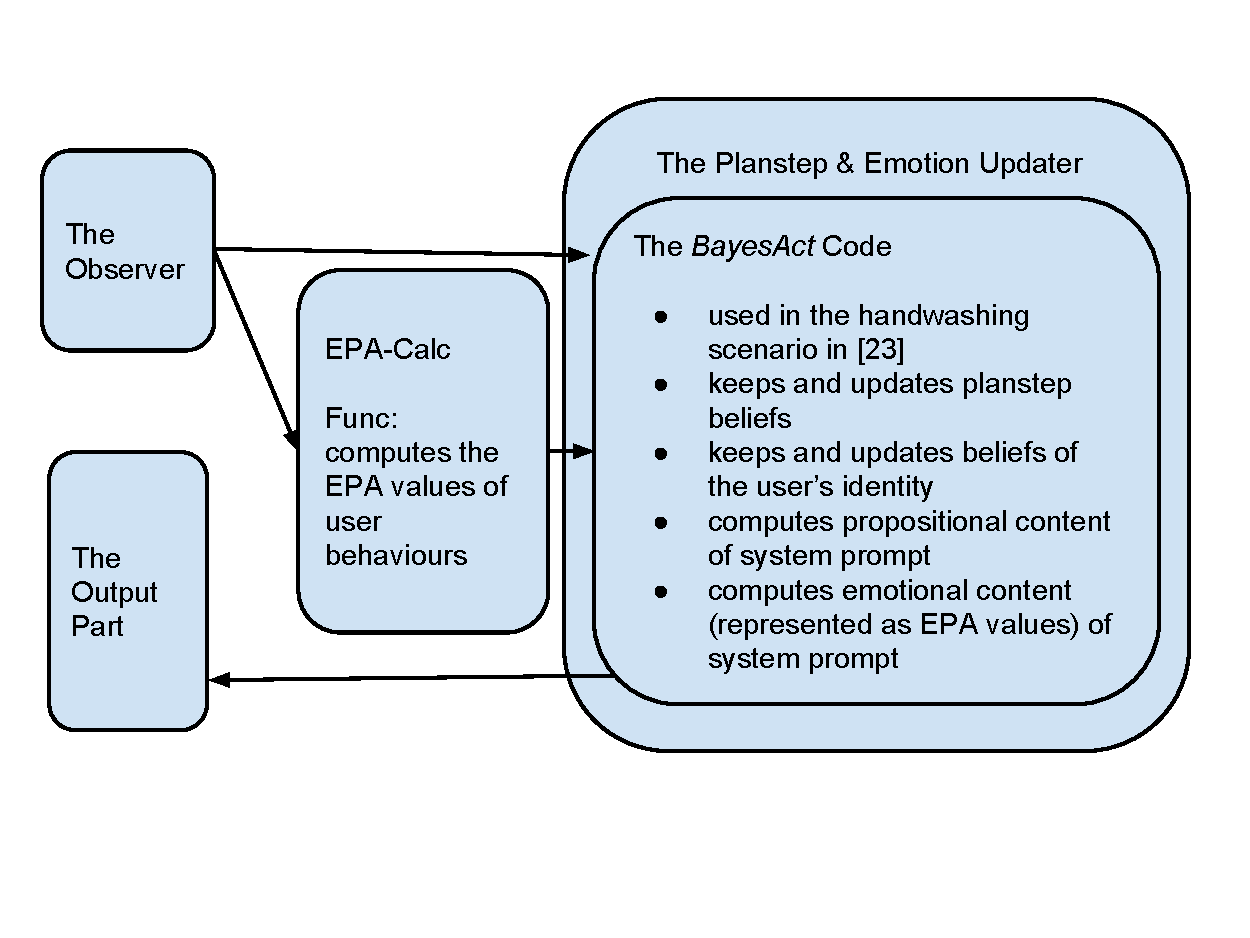
\includegraphics[trim = 4mm 30mm 5mm 15mm, clip, width=0.9\linewidth]{fig/fig-updater.pdf}
\caption{Design the planstep and emotion updaters based on the BayesAct code}
\label{fig:updater}
\end{figure}


\begin{table}
\centering
\caption{Some of the parameters that need to be set when using the BayesAct engine}
\label{table:bayesact-param}
\begin{tabular}{| l | l | p{9.4cm} |}
\hline
param & default value & meaning \\ \hline
$\beta_{a}^{0}$ & $0.01$ & initial identity variance for agent (larger means agent is more uncertain of its own identity) \\ \hline
$\beta_{c}^{0}$ & $0.01$ & initial identity variance for client (larger means agent is more uncertain of the client's identity) \\ \hline
$\gamma$ & $(1.0, 1.0, 1.0)$ & model noise variance of the E, P, and A values of user behaviours (larger means agent is more uncertain of the input) \\ \hline
$N$ & $300$ & number of samples used in the computation \\ \hline
$f_a^{0}$ & $[1.5,0.51,0.45]$ & the agent's initial belief of its own identity \\ \hline
$f_c^{0}$ & $[1.59,0.79,-0.88]$ & the agent's initial belief of the client's identity \\ \hline
\end{tabular}
\end{table}

Recall that the BayesACT model includes states $S = \{X, F, T\}$, observations $\Omega = \{\Omega_{x}, \Omega_{b}\}$, and agent actions $\{A, B_{a}\}$. In our hand-washing system, $X = \{X_{turn}, X_{ps}, X_{aw}, \\ X_{bahav}\}$, where $X_{turn}$ describes whether the agent or the client is acting at this time, and $X_{ps}$, $X_{aw}$ and $X_{bahav}$ represents the current planstep, awareness and behaviour of the client. The observation $\Omega_{x}$ gives evidence to the system about $X$, including evidences indicating which party is currently acting, and what behaviour the client is currently performing if it is currently the client's turn. The system action $A$ denotes the propositional content of a system message. For example, it can be ``to instruct the user to rinse his hands''. The observation $\Omega_{b}$ gives evidence to the system about $f_b$, which is an attribute in $F$ representing the estimation of the affective meanings of the client's behaviours (when it is the client's turn). The observation function for the client behaviour sentiment $Pr(\Omega_b|f_b)$ is defined. It allows one to specify the ``confidence'' or ``reliability'' of the different components of $\Omega_b$ by $\gamma$, which is the variance of a normal (Gaussian) distribution (see Table~\ref{table:bayesact-param} and also the start of Section~\ref{sec:impl-epacalc}). $B_{a}$, whose value is an EPA vector, denotes how the message should be expressed. For example, it can be ``state the instructional message with a friendly tone''. 

A definition of eight plansteps is used to describe different functional states of the user in a hand-washing process. The corresponding planstep update diagram of this definition is shown in Figure~\ref{fig:planstep}. The current planstep belief $X_{ps}$ is a discrete variable with eight values (states), where the $i$-th state denotes the probability of the system currently being at planstep $i$. Two probability distributions are used to compute the $X_{ps}$ transitions given an observation of the user's behaviour: the distribution $Pr: X_{behav} \to \Delta(\Omega_{x})$ of the user's behaviour over behavioural observations, and the distribution $Pr: (X_{ps}, X_{behav}) \to \Delta(X_{ps})$ of the user's functional state moves from one planstep to another after a certain behaviour is performed. $X_{aw}$ is a binary variable. It describes if the user is aware or not. A variable $D$ is used to describe the current emotional deflection in the interaction and to infer how responsive a person is to a prompt. $D$ corresponds to the differences between $F$ and $T$. The dynamics in the system are: \\
--- If the user is aware (i.e. has a high $X_{aw}$ value), then if there is no prompt from the agent, the user will advance stochastically to the next planstep with a probability that is dependent on the current observation of user behaviour and the deflection $D$. If the user does not advance, she loses awareness (i.e. has a low $X_{aw}$ value). \\
--- If the user is aware (i.e. has a high $X_{aw}$ value) and is prompted, and the deflection $D$ is high, then a prompt will likely confuse the user and cause him/her have a low $X_{aw}$ value. Again, this happens stochastically. \\
--- If the user is not aware (i.e. has a low $X_{aw}$ value), then if there is a prompt from the agent, and the deflection $D$ is low, the user will likely follow the prompt, which causes the $X_{aw}$ value to rise. Otherwise (i.e. there is no prompt, or the deflection $D$ is high), the user will not do anything (or do something other than the one prompted) with high probability.


\section{The EPA-Calculator}
\label{sec:design-epacalc}

The BayesACT model does not tackle the problems of affect recognition and generation. Thus, for it to be used, an ``input mapper'' measuring the EPA values of user behaviours, as well as an ``output mapper'' mapping the propositional and EPA-vector descriptions of the system's guidance messages into concrete prompts are needed. The ``input mapper'' corresponds to the EPA-Calculator discussed in this subsection, and the ``output mapper'' corresponds to the Output Part of the system, which will be discussed in Section~\ref{sec:design-output}.

The problem of affect recognition from human behaviours, including affect recognition from bodily movements, facial expressions and sentences spoken, is a difficult machine learning problem. Chapter~\ref{chap:bg} of this thesis reviewed some of the previous work in recognizing affect from user behaviours; however, constrained by the specialty of our application scenario --- to assist people with dementia (i.e. special user group) during hand-washing process (i.e. special use case where user's verbal and facial expressions can not be obtained easily and/or clearly) few of the previous approaches fit into our system naturally.

Recognition studies from facial expression analysis, which are relatively mature approaches, are not suitable for our application scenario. There are several reasons for this. Firstly, most facial expression analysis methods are based on data sets consisting of acted expressions; even though for approaches where spontaneous expressions are used, the expressions are performed by normal, healthy persons rather than persons with dementia, the user group of our hand-washing system. Since diseases could cause physical changes (e.g. persons with dementia might have fewer facial expressions), the performance of the facial expression analysis methods claimed to have high accuracies elsewhere might not remain the same when applied to our application. Moreover, most existing approaches analyse clear front-view facial expressions, which are difficult to obtain during the handwashing process. 

Studies have as well examined acoustic-based methods that recognize affect by analyzing acoustic features, words spoken, or even sentence structures. However, speech recognition for elderly persons is harder than for younger people, and dementia can cause additional difficulties. Also the ambient noises (e.g. water running) can be a possible problem. Thus it is not feasible to collect user voices clearly during the hand-washing process, not to mention that extracting and analyzing words selected and sentence structures from audio recordings is itself a big challenge. 

One possible approach to deal with the user-group constraints of our application is to select features by cooperating with sociologists, psychologists and physiologists, and to collect and label data. However, the approach requires a large amount of time, effort and expertise. With its focus on building a prototypical system integrating emotional intelligence, this thesis project leaves this for future work.

In our approach, the expansiveness between user's hands and the velocity of the user moving his/her hands are the features chosen in the system for computing affective meanings (potency and activity, to be specific) of user behaviours. This selection is supported by previous studies. For example, in the work of Beck and his colleagues \cite{beck2010interpretation}, the authors derived a relationship between motion parameters and affective state, and showed that velocity and expansiveness correlate with arousal.

Threshold-based approaches are used to map expansiveness and velocity levels to potency and activity values of the EPA vectors representing a user's behaviours. The evaluation value of the EPA vector remains as default values in this prototypical approach. The calculated EPA representations are then fed into the Emotion Updater where the system's belief states about the user's identities are updated. Based on the belief states, the Emotion Updater then produces the affective meanings required for system prompts according to the principle of minimizing deflection. The EPA-Calculator is designed and implemented as an independent component from the Emotion Updater, which makes it easy to improve the calculator's performances by adding more features or employing new machine learning models without affecting the design of the Emotion Updater and other components in the system.

\section{The Observer}
\label{sec:design-observer}

The Observer perceives the world by sensors. What sensors should be mounted and what information should be extracted depends on the input requirements of the Planstep Updater and the EPA-Calculator. Concluded from the discussions in previous sections, the functionality of the Observer is to detect user behaviours (required by the Planstep Updater) and to compute expansiveness and velocity of the user's hand movements (required by the EPA-Calculator). Our design uses location-based methods to produce these features from hand locations. Figure~\ref{fig:location-use} shows how this is done.

\begin{figure}[htp]
\centering
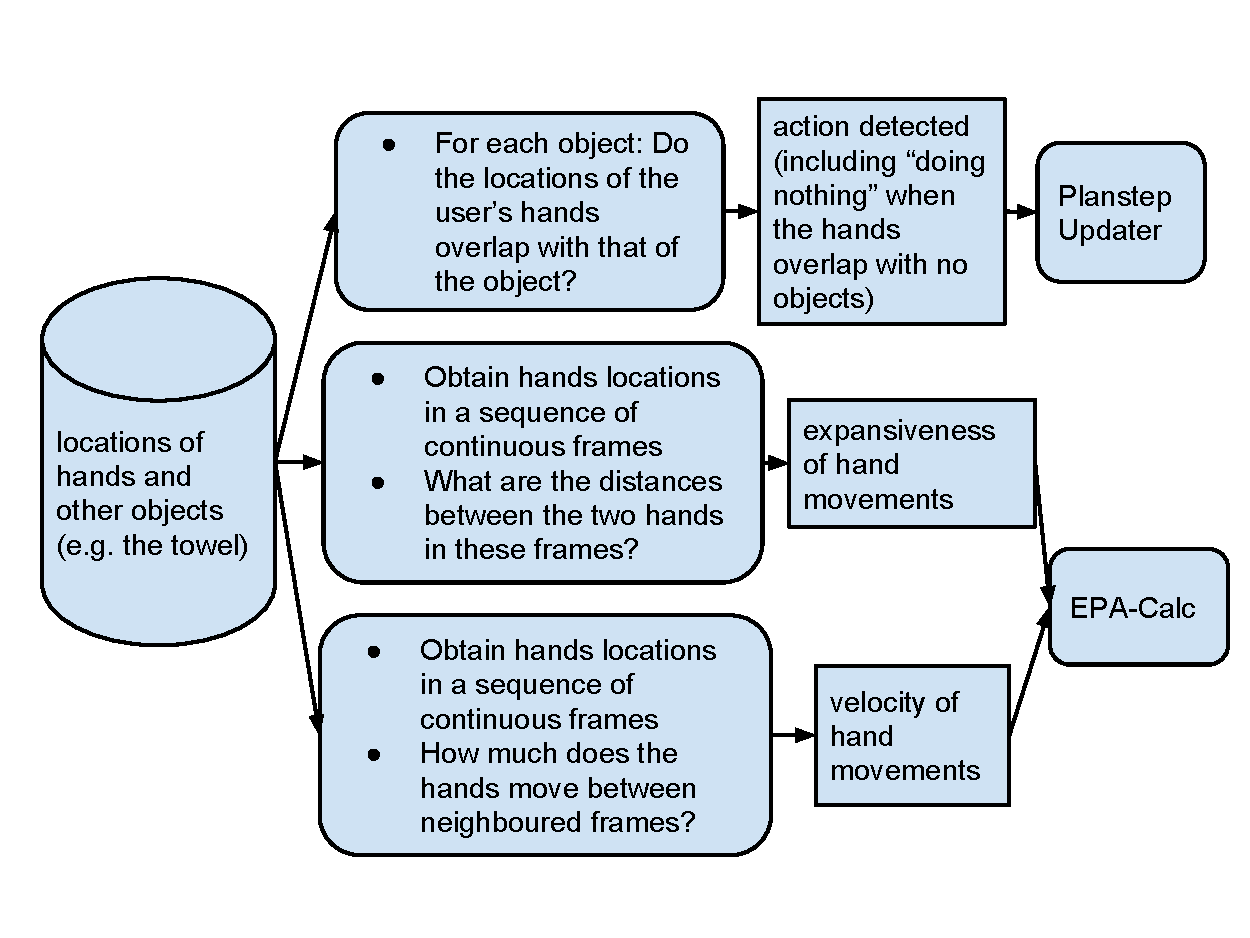
\includegraphics[trim = 4mm 13mm 2mm 14mm, clip, width=0.9\linewidth]{fig/fig-location-use.pdf}
\caption{How the location info of hands and other objects are used in the system}
\label{fig:location-use}
\end{figure}

As shown in Figure~\ref{fig:location-use}, location-based methods detect user behaviours by comparing the locations of the user's hands with those of the objects we are interested in (as in \cite{boger2005decision, czarnuch2014}). With pre-defined coordinates of certain objects (e.g. the soap, the towel, etc), a user behaviour (e.g. ``using the towel'') is said to be detected if the corresponding object (e.g. the towel) is close to the user's hands. If multiple objects are close to the user's hands, then the closest one is said to be selected. Apparently, the range at which the hands are considered ``close enough'' to an object should be designed carefully. For example, the ranges should be different for different objects. 

To be more sophisticated, as opposed to being a constant value, the range associated with an object in a location-based method could even be implemented as a probability distribution describing the probability of the user's hands touching the object given the distance between the coordinates of hands and the object. In such a case, comparisons between distances would become comparisons between probabilities, and the object that is closest to the user's hands would become the one that has the highest probability of being touched by the user. In the work of Hoey and Poupart \cite{hoey2005solving}, the authors described the probability distribution of user behaviours given hands locations directly as a POMDP observation function. In their approach, given observations of continuous x-y-z positions of the user's hands, the probability distribution of user behaviours was computed by the observation function, which was some Gaussian distribution.

Location-based approaches of detecting user behaviours have their limitations, in the sense that observing the user's hands at a position does not necessarily imply that the user is performing a certain behaviour. Including context information, such as which planstep the person is currently at, or utilizing additional sensors, such as ones that can detect water flow changes, might improve the accuracy of behaviour detection for location-based approaches. However, requiring too many sensors is undesirable for a system assisting people with everyday tasks. Luckily though, since the Planstep and Emotion Updater is designed and implemented as a POMDP in our system, all this uncertainty of observations is gracefully handled.

As mentioned above, essentially, the Observer needs to recognize the user's hands from grabbed images and obtain the coordinates of the hands. Chapter~\ref{chap:bg} of this thesis reviewed some previous work in tracking human hands, among which Czarnuch and Mihailidis's approach utilized the depth information of images \cite{czarnuch2014}. Their tracker is able to recognize and track the user's hands accurately and is a suitable base for the Observer component of our hand-washing system. Chapter~\ref{chap:impl} of this thesis gives a more detailed explanation on the accuracy of the tracker recognizing user's hands. This thesis designs the Observer component of the system as an extension to the tracker developed by Czarnuch and Mihailidis in their work. The coordinates of a set of objects, which are the soap, the towel, the taps, the sink and the running water, are predefined. 

The Observer of our system uses an RGBD camera mounted above the sink area to grab images and extract features of the user's hand movements. A 4D camera is better than a normal camera in the sense that it is able to get depth information of objects as well. With this additional information provided, image analyzers are able to achieve more accurate results. In fact, it would be difficult for the analyzers to differentiate the vertical distances between the user's hands and certain objects without depth information, in which case the user would be detected as ``using the soap'' whenever his/her hands and the soap are projected at the same place on the x-y plane (regardless of what the z values are). 

\section{The Output Part}
\label{sec:design-output}

A prompt is an instructional message the handwashing system gives out suggesting what the user should do next. As discussed before, in order to convey the intent of the instructions effectively to its user, the system should carefully decide how it should express the instructions. That being said, a prompt is defined with two components: the proposition and the emotion. The propositional part represents ``what behaviour the user should perform next'', while the emotional part indicates ``how the instructional message should be expressed''. Two prompts are considered identical only when they contain the same propositional content and are expressed with the same emotion. For example, the audio messages ``please turn on the water'' and ``please put on some soap'' are different prompts, since they contain different propositional contents. The audio messages ``put on some soap now you slowpoke!'' and ``could you please put on some soap?'' are different prompts as well, since they have different emotional interpretations.

While the main functionalities of the updaters are to update the belief states of the user's planstep and emotional state, they also compute the propositional (i.e. what instructions should be given) and emotional (i.e. how the instructions should be expressed) descriptions of prompts. The descriptions are then fed into the output part, where final prompts are either selected from predefined prompt sets or generated dynamically. This falls into the category of affect generation. The output part also displays the final prompts if needed. Note that prompts might not be needed at every timestep. In fact, if the user is performing smoothly by himself/herself, he/she might even get interrupted and confused by prompts. For easier descriptions, an ``empty prompt'' is defined to describe situations where no prompt is needed.

Dynamic generation of affective messages is a large challenge, as exemplified by the literature on embodied conversational agents (see \cite{cassell2000embodied, niewiadomski2013computational}, and Chapter~\ref{chap:bg} of this thesis). Our approach selects the final prompt to display to the user from a set of pre-generated and evaluated prompts. The four most essential questions involved in this approach are: (1) Deciding the format of the pre-generated prompts: should they be video, audio, or textual prompt? (2) Designing the prompts, e.g. the words used in the prompts. If the prompts are audio or video prompts, the tones how the messages are stated should be carefully designed as well. Character gestures and other details might require consideration as well if video prompts are used. (3) Labeling the generated prompts. While it might be easy to label the propositional content of the prompts, labeling the emotional interpretations of the prompts might require additional effort. (4) Selecting the prompt to display based on the propositional and emotional descriptions at each timestep. 

The effectiveness of different prompt formats depends on many variables, including personal preference and physical states of the users. For example, some users might find that videos with more information encoded are more helpful, while some others might not even look at the screen. The performance of prompt formats depends on the users' physical states as well. Ideally, the system should learn users' responsiveness to different prompt formats and select the most appropriate ones, or allow users to set prompt format preferences themselves. The format of audio-visual is used for the purpose of demonstration in our prototype. The format of audio-visual was used in the previous work on COACH system as well \cite{mihailidis2008coach}.

Prompt design is very important as it directly affects the usefulness of the prompt. The user would have difficulty understanding the system's intent if an ambiguous prompt is displayed. Aside from stating its intent clearly, the system should also encode emotion in the prompts. For example, different character gestures should be used to infer to different emotional interpretations. The more prompts with different emotional interpretations are generated, the more choices from which the final prompt is selected are provided and the more accurate results are expected. However, the number of pre-generated prompts is limited. Thus, the number of prompts pre-generated and the emotional interpretation differences between the prompts both need to be carefully decided. 

This thesis uses the set of audio-visual prompts generated and evaluated in Malhotra's study \cite{malhotra2014} as a prompt dataset and selects the most proper prompt from it. Malhotra designed 30 emotionally aligned audio-visual prompts that could be used by a cognitive assistive system in a handwashing scenario in her study. An empirical survey was conducted by Malhotra to get the prompts evaluated in terms of EPA values. Readers can refer to Chapter~\ref{chap:bg} for more details of Malhotra's study. Given the set of pre-generated video prompts with both propositional and emotional labels, and the propositional and emotional descriptions of desired prompts computed by the Planstep- and Emotion-Updater, the Output Part is able to select a most proper prompt from the set by choosing the prompt with the same propositional labels and the closest emotional (EPA) values from the pre-evaluated set. The difficulty of the selection then lies in the definitions of emotional closeness between prompts. The emotional closeness of two prompts is related to the Euclidean distance between their emotional labels (i.e. the EPA vectors representing their emotional interpretations). Readers can refer to Chapter~\ref{sec:impl-output} of this thesis for more details of the algorithm used in our approach to choose the final prompt from the prompt dataset.

After a most proper prompt is chosen, the Output Part displays it out to the user. The sub-component that serves as a multi-media player in the Output Part is designed as a VLC\footnote{An introduction to the VLC SDK can be found via \url{https://wiki.videolan.org/LibVLC/}.} SDK application. VLC SDK is a mature and easy-to-use media framework that can be embedded into systems to provide multimedia capabilities for the applications. Minor implementation details, such as the timings to display prompts (e.g. the minimum time length between displaying two prompts), should be decided carefully.

\section{Communication between Components}
\label{sec:design-commu}

In our system implementation, if an open source package is used, it is used as is (of course, with some interface wrappers if necessary), which means that it has not been rewritten in languages different from their original implementations or been rewritten into APIs. There are several reasons for this. Firstly, the original implementations are usually stable. These widely distributed open source packages have already been tested by the developers who developed them and a large number of users who used them. Secondly, it is easier to extend or maintain the handwashing system by using the open source packages as is. In this way, one can easily update the system by replacing the plug-ins to newer versions (possibly with some changes to the interfaces), whenever bugs are found and fixed in the packages, better performance is achieved by newer implementations of the packages, or more suitable packages are found. Thirdly, it saves time and effort to use the packages as what they are. To sum up, using existing packages without modification is safe, easy to maintain, extend and switch to other packages if needed, and effort-saving.

\begin{figure}[htp]
\centering
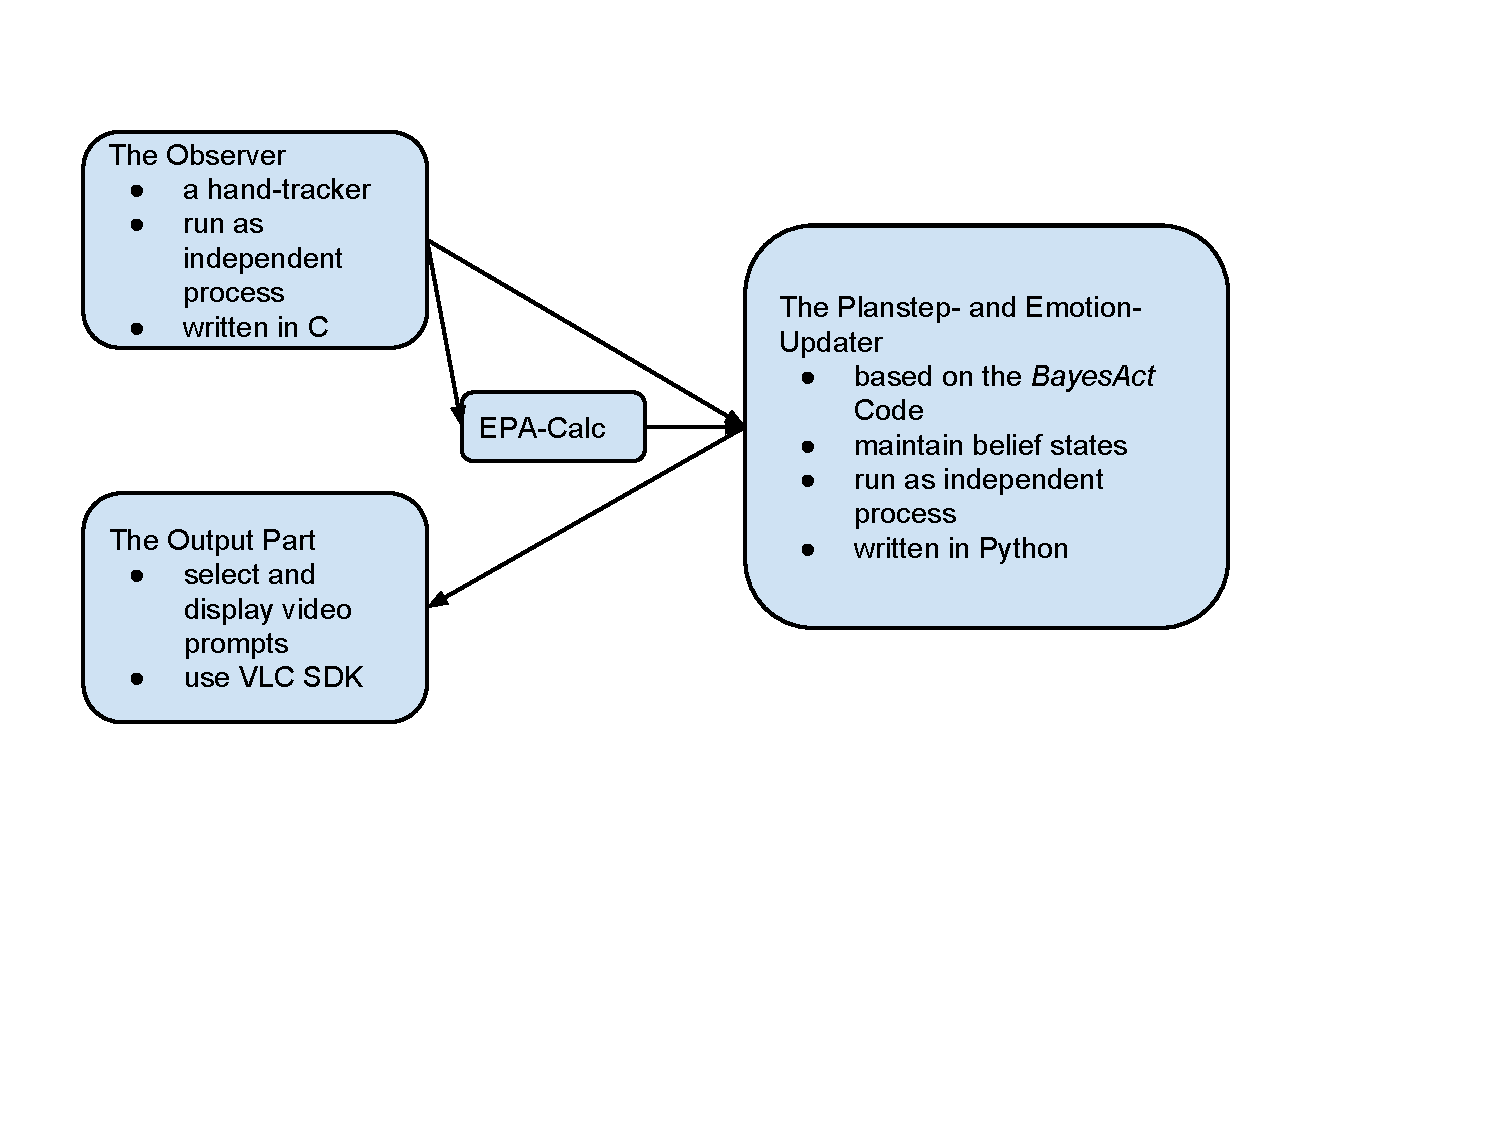
\includegraphics[trim = 10mm 63mm 37mm 20mm, clip, width=0.9\linewidth]{fig/fig-dataflow.pdf}
\caption{Data flow and logical relationship between components}
\label{fig:dataflow}
\end{figure}


Figure~\ref{fig:dataflow} shows an overview of how the system is designed as independent components. Note that different components of our hand-washing system utilize different techniques (e.g. developed using different languages) and work differently (e.g. run as an independent thread v.s. serving as an API or component). Specifically, the Observer component is designed as a hand-tracker based on Czarnuch's tracker \cite{czarnuch2014}, where the original tracker was implemented in C. The Planstep- and Emotion-Updater is designed based on the BayesAct framework \cite{hoey2013bayesian} which was written in Python. Therefore, coordination between these components is a problem. 


\begin{figure}[htp]
\centering
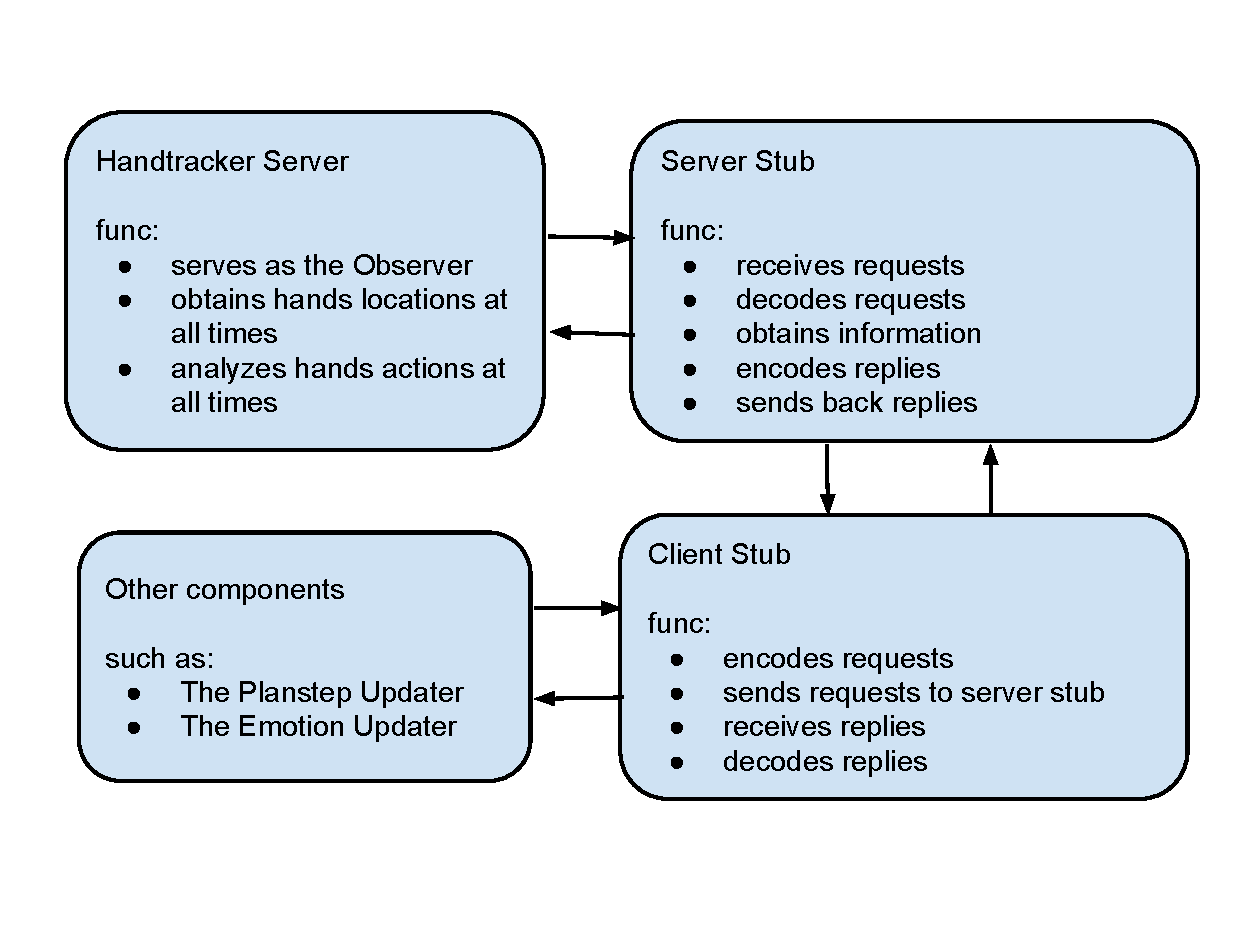
\includegraphics[trim = 6mm 22mm 6mm 18mm, clip, width=0.9\linewidth]{fig/fig-communication.pdf}
\caption{Communication between components using server-client model}
\label{fig:communication}
\end{figure}

The server-client model is utilized in our approach. A server stub and a client stub are developed on both communication parties to encode, send, receive, and decode messages for the two parities. Figure~\ref{fig:communication} shows an example of employing the server-client model in a scenario where a Hand-tracker Server that tracks the user's hands at all times is employed as the Observer component. The definitions of the request and response messages used in the communications should be shared by and accessible to both the  the server and the client stubs. One way to achieve this is to define message structures on both the client and the server side, and manually ensure that the definitions are identical. This approach is easy to implement; but is vulnerable to bugs and is difficult to maintain. Another approach is to defined the message structures within a single ``header'' file accessible to both of the two sides. The ``header'' file should be referred to in the implementation of both the client and the server side. This approach is safer than the first one in the sense that no manual effort is needed to ensure the consistency of messages definitions on the two sides. However, it is infeasible to share same ``header'' files between two components implemented with different languages. A more sophisticated approach, which is also our approach, is to use Google's protocol buffer mechanism\footnote{Introduction to the mechanism can be accessed via \url{https://developers.google.com/protocol-buffers/}.}, which allows one to define message structures at one place, and to use them at another place. By compiling and automatically generating the definitions in another language, this mechanism ensures the consistency between message definitions shared by both of the communicating sides. The mechanism is also convenient to utilize. It is able to define data attributes in a structure as ``repeated'', ``optional'' and ``required'' fields, which is beneficial to define complicated data types. Useful accessible functions to data fields are provided by the mechanism. Furthermore, since the consistency between message definitions are automatically ensured, message structures defined using this mechanism are extensible.

The timings of the client requests and the server replies are carefully decided. The components shown in Figure~\ref{fig:dataflow} work with different frequency: the Observer recognizes user's hands, obtains and analyzes hand locations for each frame grabbed by the sensor at a rate about 24 frames/second , while the Updater works as a turn-taking model between the agent (i.e. the system) and the client (i.e. the human user). Our solution to solve this problem is to use a buffer between the Observer and the Updater. Information (such as hand locations) obtained from the Observer is saved and analyzed in the buffer. EPA values of user behaviours computed by the EPA-Calculator are stored as well and can be temporally smoothed in the buffer. The algorithm the Buffer uses to temporally smooth the EPA values of user behaviours is explained in Section~\ref{sec:impl-epacalc}. Messages are sent to the Updater for state updates only when certain conditions are met. 

The following three aspects should be carefully designed for the buffer: (1) the conditions which would trigger the buffer to transfer between states; (2) the buffer's size, i.e. the information processed for how many frames can be handled by the buffer; (3) the policy describing how overflowed messages are dealt with. The state machine shown in Figure~\ref{fig:state-trans} illustrates how the buffer is designed in this thesis. As shown in the figure, there are three states of the buffer. State A represents the state where the user performs a same user behaviour within neighbouring frames. Two conditions can trigger the buffer's state to transfer from State A to another state: (1) If a user behaviour different from the current stable behaviour is detected, then the state of the buffer would transfer to State B. If the new behaviour is found to last for less than a \textit{timeup} period, the state of the buffer would change back to State A, with the stable behaviour unchanged. (2) If the buffer has been in State A for a \textit{timeout} period, then the buffer would change to State C, where the state of the buffer would change back to State A immediately after messages encoding the current stable user behaviour are sent to the updaters. State B of the buffer checks if a newly detected user behaviour is a stable one. Similarly, there are two conditions that can trigger the buffer's state to transfer from State B to another state: (1) If the new user behaviour different from the current stable behaviour is found to last for at least a \textit{timeup} period, then the new user behaviour is considered stable. In that case, the state of the buffer would change to State C, where the buffer's state would change to State A immediately after messages encoding this new stable behaviour are sent to the updaters. (2) Otherwise, the buffer's state would change back to State A with the current stable user behaviour non-changed.

\begin{figure}[H]
\centering
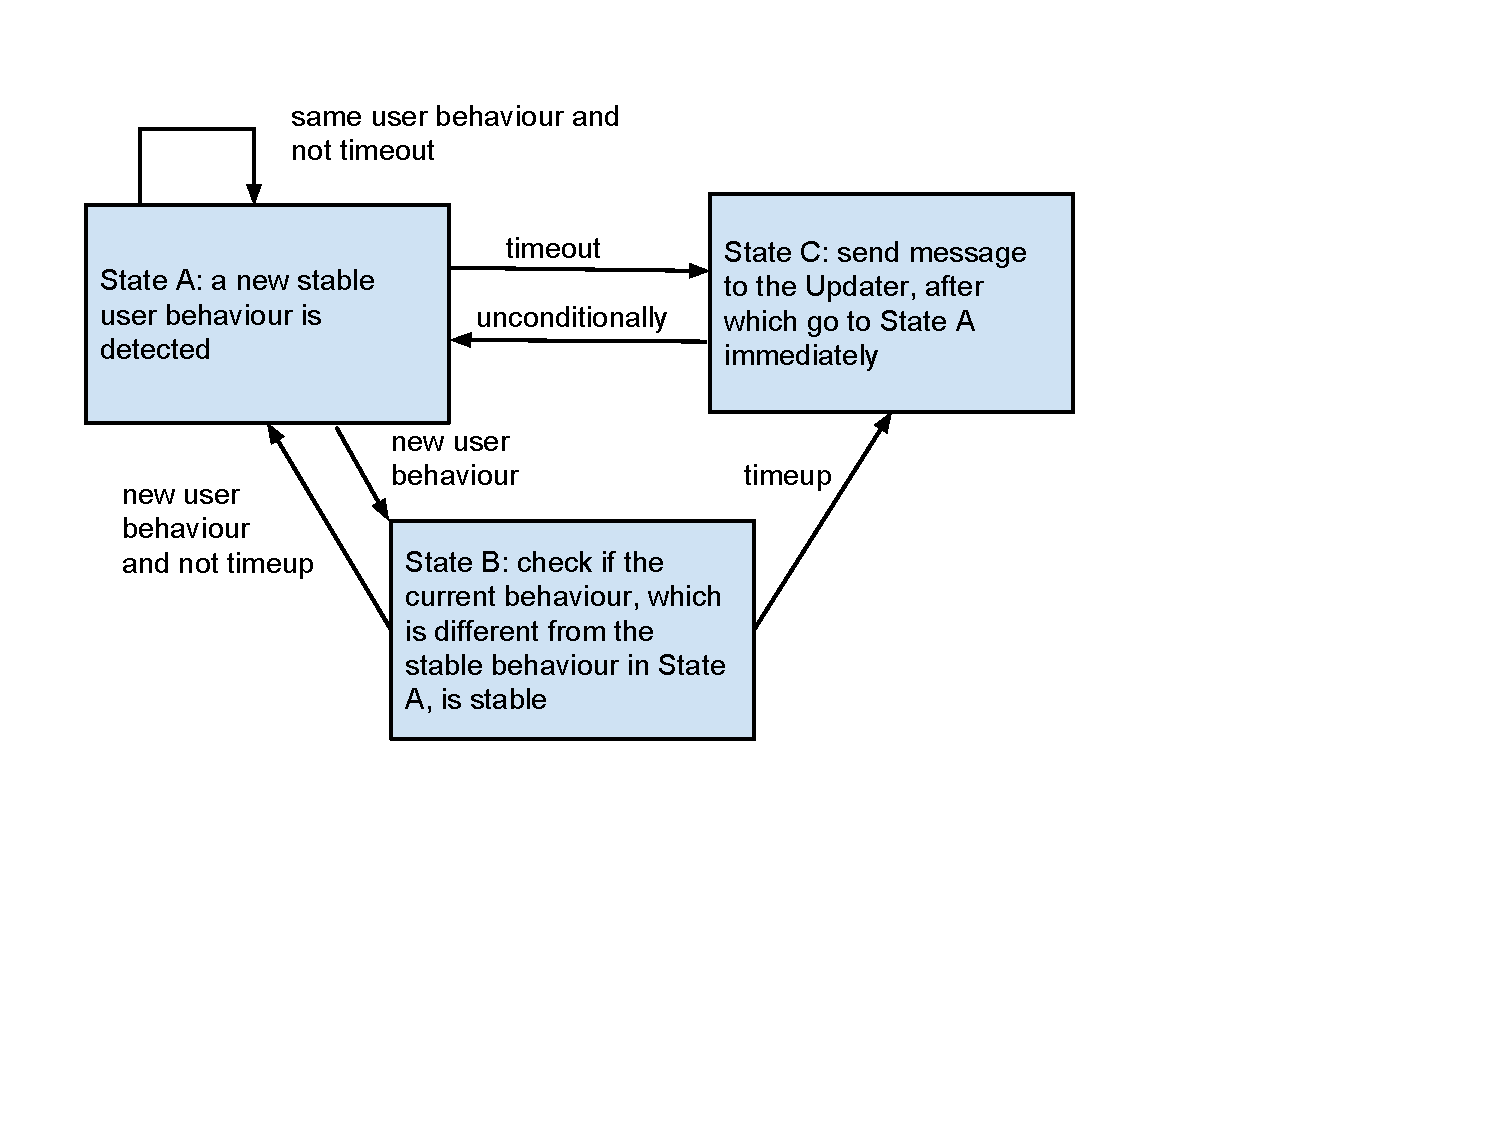
\includegraphics[trim = 10mm 60mm 50mm 17mm, clip, width=.85\linewidth]{fig/fig-state-trans.pdf}
\caption{State transitions of the buffer between the Observer and the Updater}
\label{fig:state-trans}
\end{figure}
 

\section{Summary}

\begin{figure}[h]
\centering
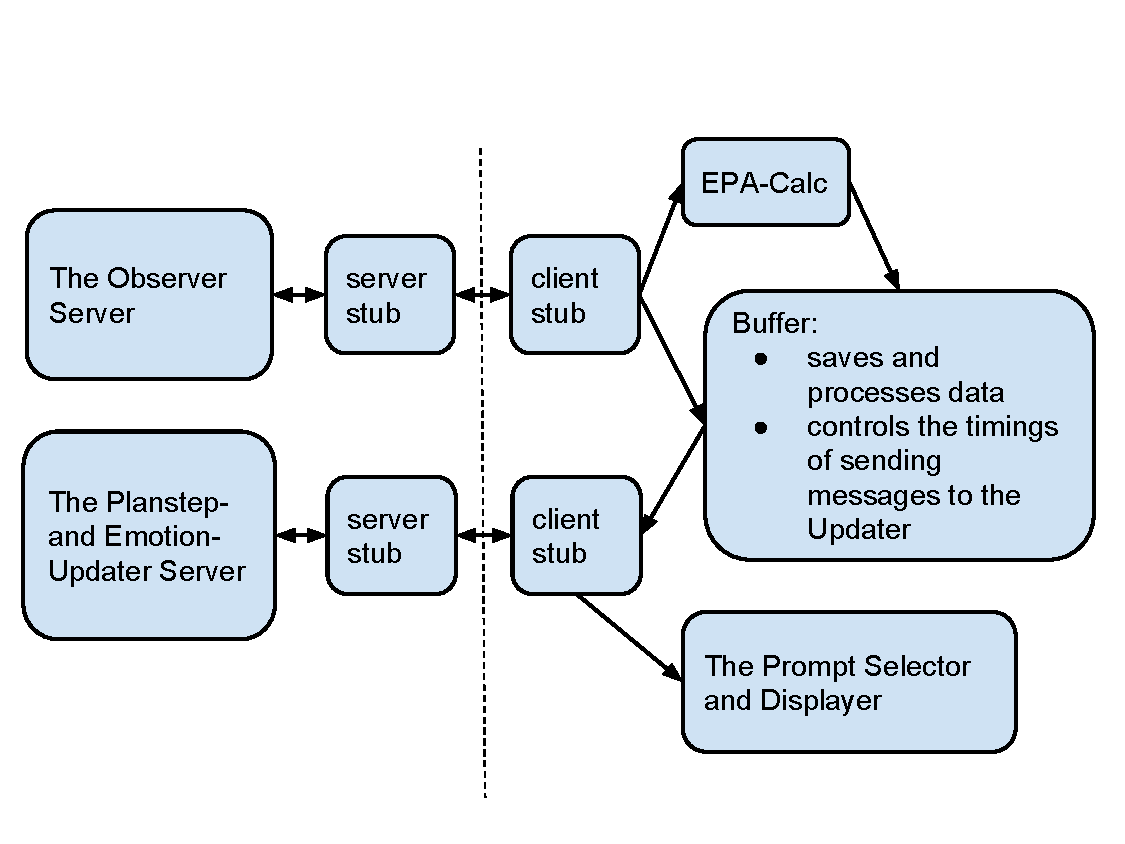
\includegraphics[trim = 0mm 15mm 0mm 20mm, clip, width=0.8\linewidth]{fig/fig-system.pdf}
\caption{System design with server-client models}
\label{fig:system}
\end{figure}

To sum up, the system is designed as shown in Figure~\ref{fig:system}. The Observer component of the system is designed based on Czarnuch's tracker \cite{czarnuch2014}, and is used as a hand-tracker server (see Sections~\ref{sec:design-observer} and~\ref{sec:design-commu}). The Planstep- and Emotion-Updater is designed based on the BayesAct framework (implemented in \cite{hoey2013bayesian}), and is used as an Updater server (see Sections~\ref{sec:design-updater} and~\ref{sec:design-commu}. The rest of the components are designed as client components which communicate with the servers through stubs. Among all the client components, an EPA-Calculator (see Section~\ref{sec:design-epacalc}) and a Buffer (see Section~\ref{sec:design-commu}) sit between the two servers. The EPA-Calculator consumes user's hand locations and computes the EPA values of user behaviours. The Buffer stores and re-processes user behaviours and their EPA values, and controls the timings at which messages are sent to the Updater server for state changes. The final system prompt is selected and displayed by the Output Part (see Section~\ref{sec:design-output}).

Being designed as an integration of independent components, the system is easy to maintain and extend. For example, the Observer Component can be extended to obtain more features useful in computing EPA values for user behaviours without many changes to other components. This system design is portable as well. Since this design enables component communications across processes and multi-languages, one can easily use the same system design (possibly with some minor changes) in other application scenarios.



\chapter{Implementation}
\label{chap:impl}

The system was implemented by developing new modules and combining both newly-developed components and existing packages together. Most of the codes were written in C/C++, while some of it used python. Server-stubs and client-stubs were employed, and Google's protocol buffer mechanism was used as the way to define the request and response messages shared by the two communicating parties. Open source libraries, such as ZeroMQ and libVLC, were utilized as well. Each module in the system was designed and implemented in an independent, efficient, and extensible way. The rest of this section describes the system implementation in detail.

\section{The Planstep and Emotion Updater: a BayesACT reasoning engine}

We implemented the Planstep- and Emotion- Updater on the basis of the BayesAct program developed by Hoey et al. \cite{hoey2013bayesian}. In their program, a BayesAct framework that models emotional state changes during human interactions was implemented. Based on the framework, this thesis implemented a subclass of class \textit{Agent} that simulates the actions of an automated assistant in a hand-washing scenario. The subclass is called \textit{Assistant}. Class \textit{Assistant} has an attribute field denoting the values of observed behaviours, and has methods that update belief states, including $X$ and the relationships between $X$ and $Y$ (or, $F$ and $T$)), based on observations. A function to get an estimation of the ``current most-likely planstep'' was defined in \textit{Assistant} as well. The function returns the planstep that has the highest probabilities in the planstep distribution. POMDP observation functions were also defined in \textit{Assistant}. 

Noting the fact that an integer denoting the propositional messages contained in a prompt is used by both the BayesAct and the Prompt-Selector (the numbers come along with a set of predefined video prompts that the selector selects from), consistency between the two encoding systems must be assured. To achieve this, a converter on the server-stub side was implemented. The converter maps propositional descriptions of prompts returned by the server to their corresponding representations used by Prompt-Selector. Since ``turning on water'' and ``turning off water'' are denoted by same integers in BayesAct, additional information such as estimation of the current most-likely planstep is needed for the conversion. The converter is called before the server-stub packs and sends replies back to the client-stub. Relationships between the encoding systems of representing propositions used by BayesAct and the Prompt-Selector are illustrated in Table~\ref{table:prompt-number-def}.

%
% table: Mapping between action suggested in BayesAct and prompt content representations in Prompt-Selector
\begin{table}
\centering
\caption{Mapping between action suggested in BayesAct and prompt content representations in Prompt-Selector}
\label{table:prompt-number-def}
\begin{tabular}{| l | p{4.5cm} | p{4.5cm} |}
\hline
Action description & Representation number in BayesAct & Representation number in Prompt-Selector \\ \hline
no prompts needed & 0 & 0\\ \hline
ask the user to put on soap & $1$ & $2$ \\ \hline
ask the user to rinse hands & $3$ & $3$ \\ \hline
ask the user to turn on water & $2$ & $1$ \\ \hline
ask the user to turn off water & $2$ & $4$ \\ \hline
ask the user to to dry hands & $4$ & $5$ \\ \hline
tell the user all has been done & N/A & $6$ \\ \hline
Invalid/undefined prompts & N/A &$-1$ \\ \hline
\end{tabular}
\end{table}

As far as the propositional content generation policy is concerned, two options exist: a POMCP policy and a heuristic policy. The POMCP policy computes a utility function which looks several steps further to produce prompts, while the heuristic policy constructs prompts based on mappings between the estimation of the ``current most-likely  planstep'' and system actions. The mappings in the heuristic policy are obtained by heuristic knowledge and are shown in Table~\ref{table:heuristic-policy}. Considering the fact that the heuristic policy runs faster and is sufficient for our prototype system, which is used to demonstrate the feasibility of including emotional intelligence in a practical system, the heuristic policy was chosen in our approach.

%
% table: Action suggestions basing on the current most-likely planstep (heuristic policy)
\begin{table}
\centering
\caption{Action suggestions basing on the current most-likely planstep (heuristic policy)}
\label{table:heuristic-policy}
\begin{tabular}{| l | l | l | l | l |}
\hline
\multicolumn{4}{|c|}{Current Most-likely Planstep} & \multirow{2}{*}{ Actions Suggested} \\ \cline{1-4} 
Number & Soap(dirty/soapy/clean) & Water(on/off) & Hand(wet/dry) & \\ \hline
0 & dirty & off & dry & turn on water \\ \hline
1 & dirty & on & dry & put on some soap \\ \hline
2 & soapy & off & dry & turn on water \\ \hline
3 & soapy & on & dry & rinse hands \\ \hline
4 & clean & on & wet & turn off water \\ \hline
5 & clean & off & wet & use towel \\ \hline
6 & clean & on & dry & turn off water \\ \hline
7 & clean & off & dry & N/A \\ \hline
\end{tabular}
\end{table}

As discussed in the previous chapter, BayesAct is treated as a server in our implementation. Both a server-stub and a client-stub are developed. The server-stub listens to client requests at all times, and if there are any, processes them. The request processing tasks include: decoding the requests, passing arguments encoded in the request to the server for it to update belief states, and packing and replying the prompt descriptions obtained from the server to the client-stub. The client-stub packs and sends user hand-actions and EPA values of these actions to the server-stub, and waits for replies. When a reply is received, the client-stub decodes it, and converts the information accordingly, e.g. passes the information to a Prompt-Selector, where appropriate video prompts are selected.

\begin{verbatim}

message BayesactRequest {
  required double evaluation = 1 [default = 0.0];
  required double potency = 2 [default = 0.0];
  required double activity = 3 [default = 0.0];
  required int32 hand_action = 4 [default = -1];
 }
 
 message BayesactResponse {
  required double evaluation = 1 [default = 0.0];
  required double potency = 2 [default = 0.0];
  required double activity = 3 [default = 0.0];
  required int32 prompt = 4 [default = -1]; // propositional representation  
  required bool is_done = 5 [default = false]; // if reaches the last planstep
 }

\end{verbatim}

Definitions of request and response messages shared between the two communicating parties are defined using Google's protocol buffers (shown above), and the stubs are implemented using zmq libraries \footnote{The official website of the zmq library: \url{http://zeromq.org/}.}. The stubs bind or connect to given addresses in their constructors, and with the help of zmq, they are able to easily send and receive messages to/from each other. Among all the benefits that using protocol buffers and zmq brings us, the language-neutral advantage is one that is worthy of particular attention: it allows us to combine easily the BayesAct server and its stub with all other components together as a whole system, where the former ones were implemented in python, while the latter ones were implemented using C/C++.


\section{The EPA-Calculator and the Buffer: computing and temporally smoothing EPAs}
\label{sec:impl-epacalc}

Hands' coordinates obtained from the hand-tracker server are fed into an EPA-Calculator, which represents user behaviours as EPA values. In our prototypical approach, the \textit{Evaluation} of the user's behaviour in all situations are computed as a neutral value and is considered as an uninformative observation in the Emotion Updater. This is done through defining the observation function for the client behaviour sentiment $Pr(\Omega_b|f_b)$ (see subsection~\ref{subsec:design-singleengine}). To let the system neglect the $E$ value of the user's behaviour input to the Emotion Updater, we set $\gamma_e = +\infty$, where $\gamma_e$ is the attribute in $\gamma$ describing the ``confidence'' or ``reliability'' of the observation of \textit{Evaluation} of the user's behaviour. The \textit{Potency} and \textit{Activity} are computed in the EPA-Calculator based on the distances between the user's two hands within a same frame and the distances that the user's hands have moved between neighbouring frames, respectively. The $E$, $P$, and $A$ values computed for user behaviours in the EPA-Calculator are temporally smoothed in the Buffer before fed into the Planstep and Emotion Updater. The ``confidence'' of the $P$ and $A$ values computed can be expressed by setting different $\gamma$ values as well.

A parameter $n$ is used to compute the $P$ and $A$ values of the user's behaviour. The average distance between the user's two hands in a set of $n$ neighbouring frames is scaled to the $P$ value of the user's behaviour in the EPA-Calculator. The average distance $Dist[i]$ of frames $i-n+1, i-n+2, ... , i$ can be computed using the following formula:
\begin{equation}
Dist[i]=\dfrac{1}{n} \sum_{k=i-n+1}^{i}dist(positions[k,0],positions[k,1])
\end{equation}
where function $dist: Point \times Point \to real\ number$ computes the distance between two points, and $positions[k,0]$ and $positions[k,1]$ are the coordinates of the user's left/right hand in frame $k$. A piecewise linear interpolation method is used to map the average distance $Dist[i]$ to the $P[i]$, which is the $P$ value of the user's behaviour at frame $i$. Two same-length ascendingly sorted arrays of thresholds, $potency$ and $distance$, are defined. The first and the last elements of array $potency$ are $-4.3$ and $4.3$, respectively. And the first and last elements of array $distance$ are $-\infty$ and $+\infty$, respectively. The algorithm used in the mapping between $Dist[i]$ and the $P[i]$ is as following:
\begin{equation}
P[i]=(Dist[i]-distance[k-1]) * \dfrac{potency[k]-potency[k-1]}{distance[k]-distance[k-1]} + potency[k-1]
\end{equation}
where $distance[k] \geq Dist[i]>distance[k-1]$.

A set of $P$ values (say, from $P[i]$ to $P[j]$, $i \leq j$) are temporally smoothed in the Buffer to compute the final $P$ value that is fed into the Emotion Updater. The smoothing algorithm ensures that the influence of the $P[k], i \leq k \leq j$, decays with time. The smoothing algorithm used in the Buffer can be illustrated by the following formula:
\begin{equation}
P=\sum_{k=i}^{j}(\dfrac{alpha}{alpha+1})^{j-k}*\dfrac{1}{alpha+1}*P[k]
\end{equation}
where $alpha \geq 0$.
If $alpha=0$, then $P=P[j]$, which means that no temporal smoothing is used to compute the final $P$ value.

Similarly, the $A$ value of the user's behaviour are calculated based on the average of the distances his/her hands move between $n$ neighbouring frames. The average movement $Diff[i]$ during frames $i-n+1, i-n+2, ... , i$ can be computed by the following formula:
\begin{equation}
Diff[i]=\dfrac{1}{n-1}\sum_{k=i-n+2}^{i}maxDiff(positions[k],positions[k-1])
\end{equation}
where $position[k]$ contains a pair of coordinates representing the user's left and right hand locations respectively in frame $k$, and function $maxDiff: (Point_a, Point_b) \times pair(Point_c,\\ Point_d) \to real\ number$ returns $max(dist(Point_a, Point_c), dist(Point_c, Point_d))$. Piecewise linear interpolation method is used to map the average distance $Diff[i]$ to the $A[i]$, which is the $A$ value of the user's behaviour at frame $i$. Two same-length ascendingly sorted arrays of thresholds, $activity$ and $difference$, are defined. The first and the last elements of array $activity$ are $-4.3$ and $4.3$, respectively. And the first and last elements of array $difference$ are $-\infty$ and $+\infty$, respectively. The mapping algorithm between $Diff[i]$ and $A[i]$ is as following:
\begin{equation}
A[i]=(Diff[i]-difference[k-1])*\dfrac{activity[k] - activity[k-1]}{difference[k] - difference[k-1]}+activity[k-1]
\end{equation}
where $difference [k] \geq Diff[i] > difference[k-1]$.

A set of $A$ values (say, from $A[i]$ to $A[j]$, $i \leq j$) are temporally smoothed in the Buffer to compute the final $A$ value that is fed into the Emotion Updater. The smoothing algorithm ensures that the influence of the $A[k]$, $i \leq k \leq j$, decays with time. The smoothing algorithm used in the Buffer can be illustrated by the following formula:
\begin{equation}
A=\sum_{k=i}^{j}(\dfrac{alpha}{alpha+1})^{j-k}*\dfrac{1}{alpha+1}*A[k]
\end{equation}
where $alpha \geq 0$.
If $alpha=0$, then $A=A[j]$, which means that no temporal smoothing is used to compute the final $A$ value.

Note that in the computations of $P$ and $A$, variables $n$, $potency$, $distance$, $activity$ and $difference$ are used in the EPA-Calculator and $alpha$ is used in the Buffer. The values of these variables need to be set when running the system. Moreover, the number of values used to compute the final $P$ and $A$ values needs to be set in the Buffer as well. Chapter~\ref{chap:result} described a way to set the thresholds $potency$, $distance$, $activity$ and $difference$ by statistical results from experiments. In this prototypical approach, the unweighted means of distances were used and scaled to $P$'s and $A$'s; weighted average, and/or more other features can be included as indicators for the EPA values of user behaviours in future approaches.

\section{The Observer: an extension to existing hand-tracker}

Similar to the Planstep and Emotion Updater, we implemented the Observer as an extension, with a server-stub and client-stub added and several changes made to parameter values and other details, to the tracker Czarnuch developed \cite{czarnuch2014}. We explain in the following paragraphs the algorithms used in Czarnuch's tracker, the changes we made to the original program, and the implementation details of the server and client stubs. Note that a kinect camera is mounted above the sink when the Observer is in use.

In the original program, decision trees were trained on a set of images that were manually annotated to optimize key parameters. The trained tracker is then used to classify body parts in depth images grabbed from an overhead perspective. The tracker first generates a random decision forest using a simple depth feature to provide intermediate multiclass probability density functions (PDF) for each sampled image pixel. It then proposes final body part positions by aggregating the information contained in the underlying PDF. As explained by Czarnuch \cite{czarnuch2014}, the pre-trained decision trees included in their original program are able to classify body parts (including head and hands) as long as the camera is mounted from an overhead perspective to the objects and areas of interest. 

After body parts (e.g. hands) are classified, the original tracker uses a location-based method to identify ``hand behaviours''. It first checks which pre-defined areas the user's hands are currently inside of. If multiple areas are detected, then a set of rules, such as comparing the distances from the areas' centers and current hand-locations, are applied to decide the ``winner'' area that user's hands fall in at the moment. For example, suppose a ``soap area'' is defined as $(s_{x}, s_{y}, s_{z}, s_{r})$, where $(s_{x}, s_{y}, s_{z})$ are the coordinates of the area center in world space and $s_{r}$ represents the radius of this area (i.e. the area is defined as within a spherical surface). If the current left hand-location is detected as at point $(l_{x}, l_{y}, l_{z})$, where $(l_{x}-s_{x})^{2} + (l_{y}-s_{y})^{2} + (l_{z}-s_{z})^{2} \leqslant s_{r}^{2}$, then this left hand is considered to overlap with the ``soap area'', which implies an behaviour of ``using the soap''. If the user's left hand overlaps with multiple areas, then the one with a closer center to the hand's location becomes the winning area. This same ``detection of area and behaviour'' process is performed for both of the user's hands and for all pre-defined areas. Note that in this approach, the user's two hands can be detected as performing different behaviours at the same time - one using the soap within the ``soap area'' and the other one doing nothing in particular at the sink. In the Observer we developed, when different areas/behaviours are detected for the user's two hands, a function comparing the two and returning a single winning area/action is called. More details about this comparison function are explained in the following paragraphs.

%
%figure: Screenshot of Czarnuch's tracker recognizing user's head and hands
\begin{figure}[htb]
\centering
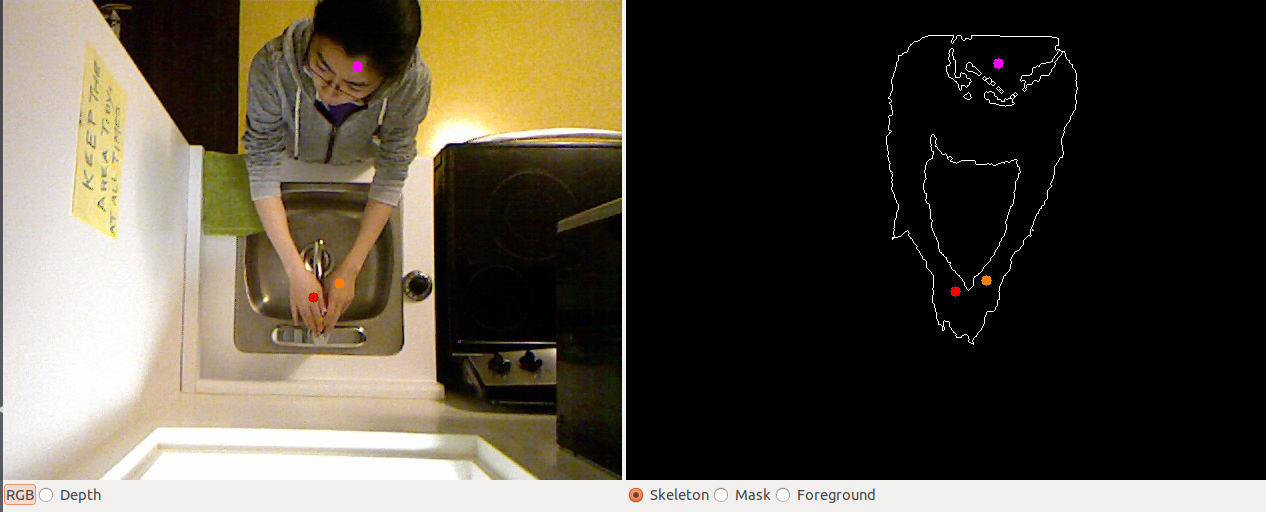
\includegraphics[width=0.9\linewidth]{fig/handtracker-performance.png}
\caption{Screenshot of Czarnuch's tracker recognizing user's head and hands}
\label{fig:handtracker-performance}
\end{figure}

Figure~\ref{fig:handtracker-performance} shows that the original tracker can recognize and return hand-positions with enough accuracy in our application scenario. Having this result, we did not retrain the model in our approach. However, if researchers were to retry our experiments, or to use Czarnuch's program in their own applications, they might need to recollect data and retrain the model. Luckily, Czarnuch included both data collection and data training modes in his program.

In our Observer, the positions and coverages of the interested areas are assigned in a configuration file. To be specific, coordinates and radiuses of seven areas, including AWAY, SINK, SOAP, WATER, Left\_TAP, Right\_TAP, TOWEL are defined. Since there was only one tap involved in the laboratory setting of our experiments (see Figure\ref{fig:handtracker-performance}), the coordinates of Left\_TAP (and Right\_TAP) are actually used to model the positions of the user's left (and right) hand when he/she tries to turn on/off the water. Priority levels to user behaviours are defined as well (see Table~\ref{table:area-action}). In the Observer, when different areas/behaviours are detected for the user's two hands, a function comparing the priority levels of two and returning the one with higher priority is called. Moreover, noticing that both the Observer and the Planstep and Emotion Updater represent areas/actions by integers, we implemented a converter function to convert between the two encoding systems to ensure that the two encoding systems are consistent with each other. Table~\ref{table:area-action} gives an overview of the relationships between areas and the user behaviours implied by them, along with the priority levels assigned to and the representations numbers used for these areas.

%
% table: Relationships between areas and the actions implied
\begin{table}
\centering
\caption{Relationships between areas and the actions implied}
\label{table:area-action}
\begin{tabular}{| l | l | p{2cm} | p{3cm} | p{3cm} |}
\hline
Area Name & Action Implied & Priority Level & 
Representation Number used in the Observer  & Representation Number used in the Updater \\ \hline
N/A & undefined action & $0$ & $0$ & $0$ \\ \hline
AWAY & doing nothing & $1$ & $1$ & $0$ \\ \hline
SINK & doing nothing & $2$ & $2$ & $0$ \\ \hline
SOAP & putting on soap & $6$ & $3$ & $1$ \\ \hline
WATER & rinsing hands & $4$ & $5$ & $3$ \\ \hline
Left\_TAP & turning on/off water & $5$ & $4$ & $2$ \\ \hline
Right\_TAP & turning on/off water & $5$ & $4$ & $2$ \\ \hline
TOWEL & drying hands & $3$ & $6$ & $4$ \\ \hline
\end{tabular}
\end{table}

As discussed previously, the Observer is treated as an observation server in our implementation. Both a server-stub and a client-stub were developed. The server-stub listens to client requests at all times, and if there are any, processes them, which includes decoding the requests, asking the server for current hand-coordinates and hand-actions, and packing and replying to the client-stub the answers. The client-stub sends requests (for current user behaviours and hand locations) to the server-stub, and waits for replies. When a reply is received, the client-stub decodes it, and converts the information accordingly (e.g. maps the representation numbers of hand-actions used by the hand-tracker to the ones used by BayesAct).

Definitions of request and response messages should be shared between the two communicating parties. With the benefit of language-neutral, platform-neutral, and easily extendable, Google's protocol buffers were used to define the message structures (shown below).

\begin{verbatim}
message HandTrackerRequest {
  optional int32 timestamp = 1 [default = -1]; // -1 means this field is not used
}

message HandTrackerResponse {
  message HandPosition {
    required float x = 1 [default = 0.0];
    required float y = 2 [default = 0.0];
    required float z = 3 [default = 0.0];
  }
  required HandPosition left_hand_position = 1;
  required HandPosition right_hand_position = 2;
  required int32 action = 3 [default = 0];
  optional int32 timestamp = 4 [default = -1];
}
\end{verbatim}

The server-stub and client-stub can be easily implemented using zmq libraries. The stubs only need to bind or connect to given addresses in their constructors, and with the help of zmq, they are able to easily send and receive messages to each other. Of course, encoding and decoding of messages should be processed according to the message definitions above before sending out and after receiving messages, respectively. The client-stub also needs to map the representation numbers of hand-actions used by the hand-tracker to the ones used by BayesAct after decoding messages.

A function called processRequestsIdle() is implemented on the server side to have the server-stub listen to client-stub requests at all times. It checks the existence of requests, and processes them accordingly if needed. The function, along with another function called handTrackerIdle(), which observes and returns hand-locations and hand-actions, are registered as the server's idle callbacks.


\section{The Output Part: Prompt Selector and Player}
\label{sec:impl-output}

Both propositional and emotional prompt descriptions are passed into a Prompt Selector, where a most appropriate video prompt is selected from a set of pre- generated and rated prompts. After this final prompt is selected, it will be sent to a Prompt Player, which was implemented by us using VLC SDK, for display. This sub-section illustrates the implementation details of the Prompt Selector and Player in order.

The set of pre-generated and rated video prompts in Malhotra's survey \cite{malhotra2014} serves as the prompt dataset for our Prompt Selector. Malhotra created these prompts using the USC Virtual Human Toolkit\footnote{See \url{http://ict.usc.edu/prototypes/vhtoolkit/}}. Figure~\ref{fig:sample-prompt} with the two screenshots of prompts instructing the user to use some soap gives a general idea of what the video clips look like. Note that the message contents of the two prompts are the same (i.e. they intend to instruct the user to do same actions); it is the way how these messages were expressed that differ them apart. The character in the first screenshot was suggesting the user to ``try putting on some soap'' with widely-open hands and a kind smiling face, giving us the impression of a nice, a little bit dominant and active lady. On the contrary, the character in the second screenshot was stating ``If you want to put on some soap, there is a soap pump lying around.'' with her hands crossed and her face unhappy. Different from the first one, the second character gives us the impression of uncaring and passive. In fact, the survey results align with our intuitive impressions: the first video prompt was rated $[1.56, 1.17, 1.35]$ for its EPA values by participants, while the second one got a rate of  $[-0.94, -0.67, 0]$ as its EPA values in the same survey.


%
%figure: Screenshots of two video prompts stating same propositional messages
\begin{figure}[htb]
\centering
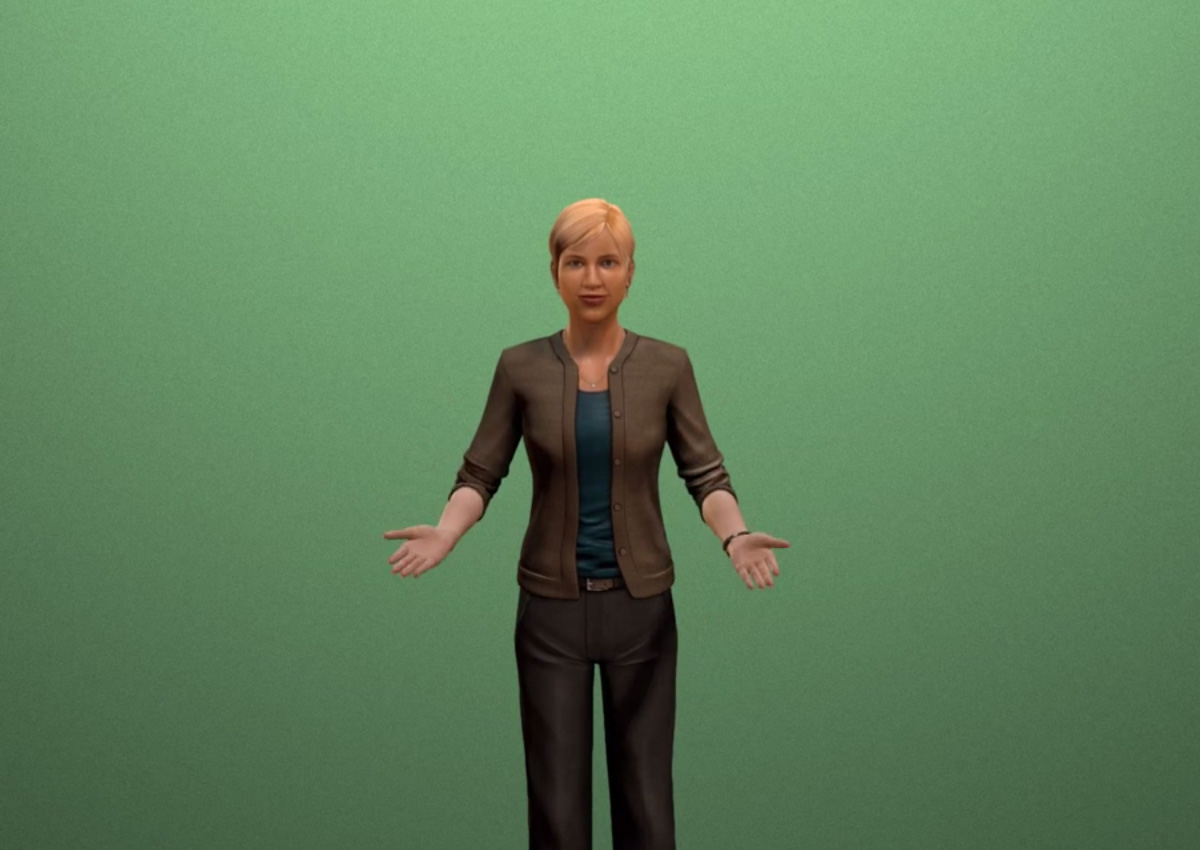
\includegraphics[width=0.45\linewidth]{fig/prompt1.jpg}
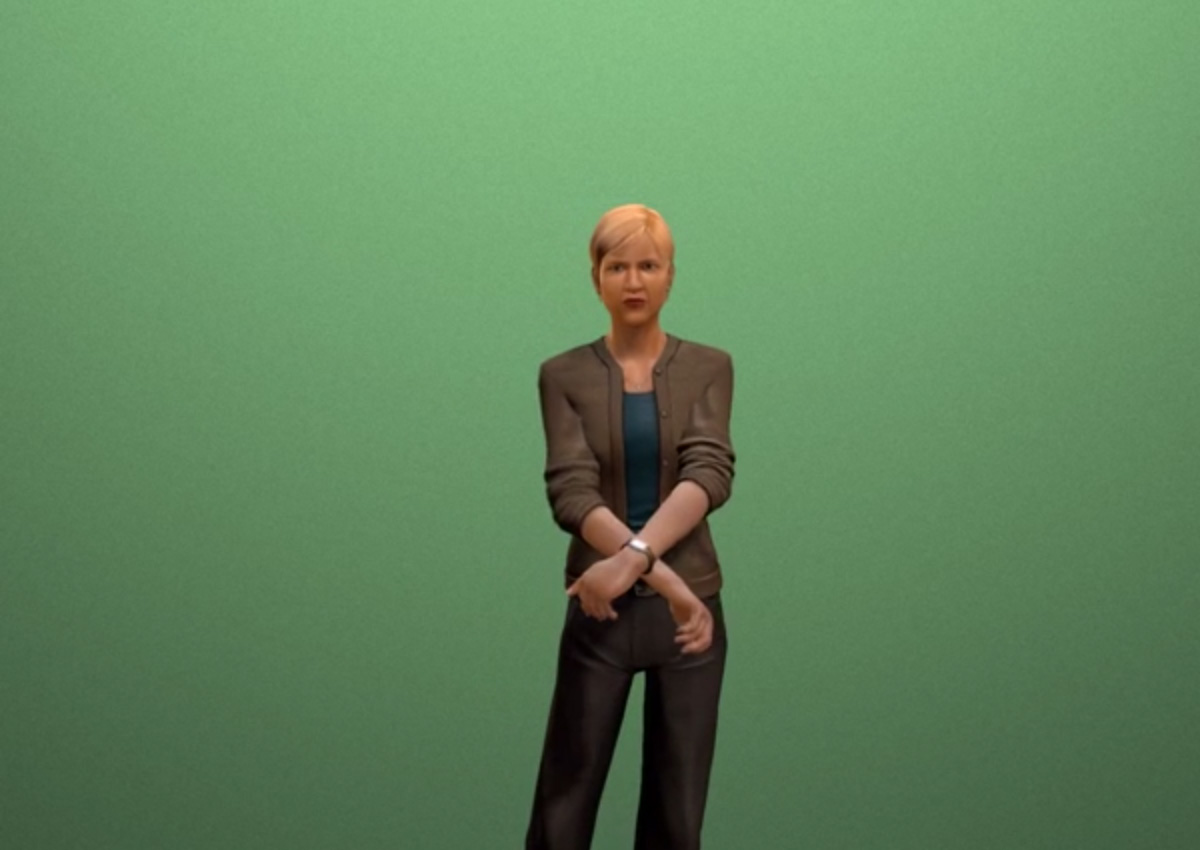
\includegraphics[width=0.45\linewidth]{fig/prompt2.jpg}
\caption{Screenshots of two video prompts stating same propositional messages}
\label{fig:sample-prompt}
\end{figure}

Each of the prompts in the dataset of the Prompt Selector has two labels: one states the propositional content of the prompt while the other one describes it emotionally. The propositional labels are assigned according to the intent of the prompts and are represented by integers. The mappings from ``intent of prompts'' to ``propositional labels'' are stated in Table~\ref{table:prompt-number-def}. The emotional labels, on the other hand, are defined as the EPA values participants rated in the survey. For example, the prompt from which the first screenshot is labelled as $[1.56, 1.17, 1.35]$ for its emotional annotation.

To utilize the pre-generated and evaluated prompts as a dataset from which the most proper prompt is selected, a file describing all these prompts (e.g. what the labels of each prompt is) is needed. When the system starts, it reads the file and stores the descriptions of prompts and their labels in memory for later use. This thesis project uses a csv file with headers ``filename'', ``prompt\_number'', ``evaluation'', ``potency'', ``activity'' to save information of the prompts. Among all the columns, ``prompt\_number'' is the integral propositional label of a prompt and ``evaluation'', ``potency'', ``activity'' are three real numbers representing the EPA values of the same prompt. 

Given the propositional and emotional descriptions of desired prompts (obtained from the BayesAct server component), the Prompt Selector is able to select the most proper prompts in the dataset via a distance-based method. To illustrate how the selector works, we first define the distance between two vectors of EPA values as the weighted Euclidean distance between them:
\begin{equation}
distance((E_1, P_1, A_1), (E_2, P_2, A_2))=\sqrt{w_E(E_1-E_2)^2+w_P(P_1-P_2)^2+w_A(A_1-A_2)^2}
\end{equation}
where $w_E$, $w_P$ and $w_A$ are weights for the three dimensions respectively. We then define the emotional distance between two prompts as the distance between their emotional annotations, i.e. the EPA values assigned to them. When given the propositional and emotional descriptions of the desired prompt, the selector selects out the video prompt that simultaneously has the same propositional label as and the minimal emotional distance to that desired prompt. In our implementation, the weights $w_E$, $w_P$ and $w_A$ are assigned values $\{1, 1, 1\}$; other values and even other definitions of the distances can be tried out in future improvements.

After the proper prompt is selected, a Prompt Player is used to display the video prompt. The Prompt Player was implemented using libVLC (VLC SDK), a mature and easy-to-use media framework that can be embedded into systems to provide multimedia capabilities for the applications.




\chapter{Experimental Results}
\label{chap:result}

Defined at the end of the Chapter~\ref{chap:intro}, the four objectives of this thesis are to augment the COACH system with an emotional reasoning engine based on BayesACT so that the augmented system: (1) is designed in a portable and extensible way; (2) runs in real-time from the perspective of the user group; (3) provides at least a level of functional assistance of as high quality as the COACH; (4) is able to tune the prompts in some way according to the emotional state of a user. It has been showed in the Chapter~\ref{chap:design} and Chapter~\ref{chap:impl} that the system we developed is easy to be extended. Experiments conducted on the system show that an average latency of 46.79ms is caused by the Observer component of the system, 0.009ms by the Buffer, and 1.65s by the Updater. The overall average latency of the system is around 1.70s, which means that the system runs in real-time from the perspective of its user group. 

We demonstrate in this section by laboratory based tests that the system is also able to provide a level of functional assistance and to produce system prompts that have encoded to some extent the emotional state of the user. The tests were conducted on a PC running 64-bit Ubuntu 12.04 LTS, with AMD FX(tm)-6300 Six-Core Processor × 6 and NVIDIA GeForce GTX 650 Ti Graphics Card. A kinect camera was mounted above the sink area and was the only sensor of the system.

\section{Parameter Setup}
This paragraph explains how the values of threshold variables $distance$ and $difference$ used in the EPA-Calculator were assigned based on statistical results obtained from experiments as follows. Videos were recorded while a person washed her hands with different emotions in nine complete hand-washing trials. A total number of 13703 frames were extracted from the videos. For each frame, the distances between the person's two hands were computed. For each pair of neighbouring frames, the distances that the person's hands moved between the frames were calculated as well. Histograms of the two ``distances'' are shown in figure 4-6 \textcolor{red}{TODO: modify this}. Note that in around 69\% of the frames, the distances between the user's hands falls into the range of $(8, 40]$. Note also that in around 70\% of frames, the distances the user's hands have moved from their positions in the last frames falls into the range of $(3.5, 17.5]$. Based on analysis of the the distributions of the two ``distances'', we assigned the values of variables used in the EPA-Calculator as following: $distance = \{-\infty, 0, 8, 40, 128, 160, +\infty\}$, $potency = \{-4.3, -4.3, 0, 1, 2, 4.3, 4.3\}$, $difference = \{-\infty, 0, 3.5, 17.5, 35, 70, +\infty\}$, and $activity = \{-4.3, -4.3, -2, -1, 0, 4.3, 4.3\}$. Table~\ref{table:param-setting} shows an overview of the values assigned to important variables in our tests of the system. 

%
% TODO: insert figure 4-6 here

%
% table: Parameter values used in laboratory experiments
\begin{table}
\centering
\caption{Parameter values used in laboratory experiments}
\label{table:param-setting}
\begin{tabular}{| l | l | l |}
\hline
\textbf{Param.} & \textbf{Value} & \textbf{Defined in which component} \\ \hline
$n$ & $10$ & EPA-Calc \\ \hline
$distance$ & $\{-\infty, 0, 8, 40, 128, 160, +\infty\}$ & EPA-Calc \\ \hline
$potency$ & $\{-4.3, -4.3, 0, 1, 2, 4.3, 4.3\}$ & EPA-Calc \\ \hline 
$difference$ & $\{-\infty, 0, 3.5, 17.5, 35, 70, +\infty\}$ & EPA-Calc \\ \hline
$activity$ & $\{-4.3, -4.3, -2, -1, 0, 4.3, 4.3\}$ & EPA-Calc \\ \hline
$alpha$ & $0$ & Buffer \\ \hline
$timeout$ & $300$ & Buffer \\ \hline
$timeup$ & $1$ & Buffer \\ \hline
$\beta_{a}^{0}$ & $0.001$ & Updater \\ \hline
$\beta_{c}^{0}$ & $2.0$ & Updater \\ \hline
$\gamma$ & $(100000, 1.0, 0.5)$ & Updater \\ \hline
$N$ & $2000$ & Updater \\ \hline
$f\_a^{0}$ & $[1.5, 0.51, 0.45]$ & Updater \\ \hline
$f\_c^{0}$ & Different in each test &Updater \\ \hline
\end{tabular}
\end{table}

\section{Overview of Two Laboratory Tests}

%
% Table: results of test #1

\begin{table}
\centering
\caption{State changes in test \#1 of the system}
\label{table:result-1}
\begin{tabular}{| V{0.9cm} | V{2.8cm} | V{1.7cm} | V{2.1cm} | V{1.7cm} | V{1.7cm} | V{2.8cm} |}
\hline

Time &
User Behaviour (screenshot) &
Behaviour prop./epa &
Planstep Belief &
f\_c &
Prompt: prop./epa &
Avatar (screenshot) \\ \hline



%column-1
t1 &
%column-2
\vskip 0.15cm
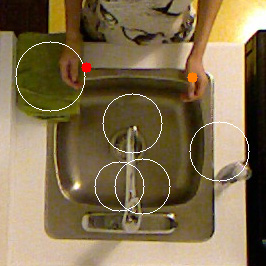
\includegraphics[width=\linewidth]{fig/system/_fast2-towel1_.jpg} &
%column-3
TOWEL
\vskip 0.2cm
$\begin{bmatrix}
0 \\
1.86 \\
-1.7
\end{bmatrix}$ &
%column-4
\begin{minipage}[c]{\linewidth} \centering
[1.00, 0.00, 0.00, 0.00, 0.00, 0.00, 0.00, 0.00] most likely planstep=0
\end{minipage} &
%column-5
$\begin{bmatrix}
1.7 \\
1.41 \\
-1.39
\end{bmatrix}$ &
%column-6
``turn on water''
\vskip 0.2cm
$\begin{bmatrix}
1.82 \\
0.22 \\
0.47
\end{bmatrix}$ &
%column-7
\vskip 0.15cm
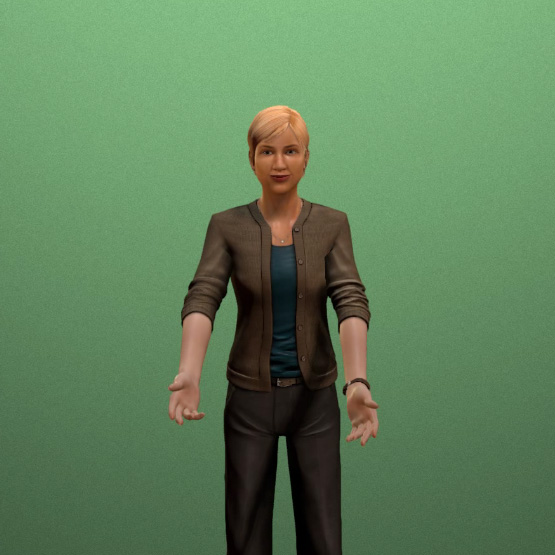
\includegraphics[width=\linewidth]{fig/prompt/_can-you-come-back-soon_.jpg}
\\ \hline



\end{tabular}
\end{table}



\chapter{Discussion}
\label{chap:discuss}

\section{Contribution}

Research in the area of emotional intelligence generally covers the following four aspects: (1) \textit{recognition of affective states}, (2) \textit{generation of affectively modulated signals}, (3) \textit{psychological study of human emotions}, and (4) \textit{computationally modelling affective HCIs}. While studies covering one or more of these aspects have been conducted, few assistive systems that have integrated all the four pieces together have been implemented. This thesis is one of the exploratory works in this area and proposed a solution to integrating emotional intelligence with a cognitive intelligent assistive system. 

This thesis defined four objectives at the beginning and sought solutions to achieve it. It reviewed previous work in all the four aspects of emotional intelligence, and designed and implemented a prototypical hand-washing system aimed at assisting people with dementia to complete hand-washing tasks successfully. As an integration of independent components, the hand-washing system is extensible and portable. The hand-washing system is able to run in real-time from the perspective of the user group, and has been shown by laboratory tests that it is capable of providing a level of functional assistance and producing system prompts that have encoded to some extent the emotional state of the user.

Approaches that can be taken to recognize affective meanings of user behaviours in the application scenario, and the difficulties that lie in those approaches have been discussed in the thesis. The author pointed out that constrained by the specialty of the hand-washing scenario and the user group of this application, vision-based approaches focusing on facial expression analysis and acoustic-based approaches, which are the two most common approaches in affect recognition, are not necessarily the most suitable solutions for recognizing affective meanings of user behaviours for this particular application. The thesis finally took an initial threshold-based approach of recognizing affective meanings of user behaviours from hand movements - to be more specific, the expansiveness between user's hands and the velocity of the user moving his/her hands. The tracker that was used to locate the user's hands was designed and implemented as an extension to an existing human body tracker \cite{czarnuch2014}.

The affective reasoning during interactions are implemented in a reasoning engine where belief state of the user's affective identities is updated basing upon BayesACT. The engine also maintains a belief state of how much the user has completed in the hand-washing process. Recommendation of prompts described in both functional (i.e. the content of an instructional message) and emotional (i.e. how the instructional message should be expressed) dimensions are produced by the engine based on the belief states and certain policies. The engine was designed and implemented on the basis of the existing BayesAct framework \cite{hoey2013bayesian}.

To enable the prompting system to display affectively modulated prompts to users, the thesis also reviewed techniques used in affective signal generation. Since dynamic generation of prompts is relatively difficult and requires much computational resources, the thesis took an approach of selecting the final prompt from a set of pre-generated and evaluated prompts. This thesis summarized that the four most essential questions involved in designing a prompt dataset and choosing a most appropriate one from it are: (1) Deciding the format of the prompts: should they be video, audio, or textual prompt? (2) Designing the prompts, e.g. the words used in the prompts. If the prompts are audio or video prompts, the tones how the messages are stated should be carefully designed as well. Character gestures and other details might require considerations as well if video prompts are used. (3) Labelling the generated prompts. (4) Selecting the prompt to display based on the propositional and emotional descriptions of recommended prompts produced by the reasoning engine. After these questions were discussed, the hand-washing system was designed and implemented in a way to select the final prompts displayed to users from a set of prompts generated and evaluated in previous work \cite{malhotra2014}. The final prompts were selected based on two conditions: (1) it should have same functional meanings as the recommended prompt by the engine, and (2) among all the prompts in the set that satisfy the first condition, it should have the smallest emotional distance, whose definition was defined in the thesis, to the recommended prompt.

Preliminary experiments where the system monitors an actor washing her hands and gives prompts were conducted. The results of two tests, where the actor behaved less powerfully and less actively in the second test than in the first, were described and compared in details in the thesis. 15 other tests of the system were conducted as well. A simple comparison of the averages of EPA values for user behaviours, the user's identities and system prompts are provided in the thesis. Detailed state changes in those experiments are provided in the appendix of the thesis. The results of the tests showed that user behaviours are roughly recognized by the system, the EPA values computed for the user behaviours are reasonable. The tests also showed that the system is able to update its beliefs of planstep and emotional state of the user, and is able to produce accordingly system prompts both functionally and emotionally. The tests also indicated that user behaviours with higher P and higher A values are more likely to lead to identity beliefs for the user with higher P and higher A values and system prompts with lower P and higher A values.


\section{Future Work}

This thesis is an initial work of integrating emotional intelligence with intelligent cognitive assistants. Our prototypical system is a first approach in this exploratory area and focuses on the integration work of combining different pieces of emotional intelligences with real-world functional assistive systems. The system may be improved in the following multiple directions:

\begin{enumerate}

\item{Improving the EPA-Calculator}

Currently, the system computes the affective meanings embedded in user behaviours based on the expansiveness of the user's hands and the velocity of the user's hand movements. By cooperating with sociologists, psychologists, and physiologists, and studying the relationships between the behaviours of persons with AD and their emotion changes, more sophisticated features/indicators may be chosen to recognize the user's emotional states. If new features are chosen, new sensors and analyzers that obtain the selected features from observations might need to be added to the system .

Data collection and labelling is needed as well to implement a sophisticated EPA-Calculator. Data can be collected by recording videos of a person's hand movements while he/she is washing his/her hands. Ideally, the behaviours of persons with dementia should be recorded in order to achieve better performance for the calculator. The number of video recordings should be designed carefully. It is desirable that the recordings cover all possibilities that how a person's emotion changes during the handwashing process, though, unfortunately, it is infeasible to achieve this in reality due to the subjective nature of emotional experiences. After videos recording people's hand movements while they are washing their hands are collected, surveys should be conducted to get these them labelled. Note that videos should be cut into shorter clips before they are labelled. This process is called data segmentation and is itself an open-ended problem. With proper segmentation, the user's emotional states (or the general emotional impressions formed by the clip) should remain stable throughout a video clip. For each short clip, a single EPA vector representing emotional impression the participant has on the clip is collected and is associated with each frame within the clip. Apparently, the time length of the video clips should not be either too long nor too short. If the video clips are too long, more than one emotions are likely to be presented by a same clip. If the video clips are too short, human raters might not be able to differentiate the emotional impressions presented by one clip from that presented by another. A solution that avoids that difficult data segmentation problem is to present the whole videos to participants, and let the participants to split and assign new EPA values to clips when they feel a new emotional impression is formed. This approach is easier to implement, with the risks of people partitioning the videos differently and unreasonably. Other aspects of the survey, such as participant eligibility for the survey, should be designed carefully as well. If the data collected and labelled is not enough, which often happens in medical research, statistical methods, such as bootstrapping, can be applied. 

Even though labelling was conducted on video clips, the labels are applied to frames within the videos, and models mapping from features extracted from the frames to the labels are trained. This is to avoid the heavy computational burden caused by learning directly from videos. Note that several frames are produced from a single video clip, and not all of them need to be included in the training process. Decisions should be made on when, how many, and what frames to cut from the video clips for training. The shorter the time period between two neighbour frames, the more accurate the result would be. However, it would require too much computational resources if neighbouring frames are too close to each other. If the frames are grabbed at a frequency higher than that at which frames are processed by the classifier, loss of data would occur as well.

\item{Improving the prompt generation process}

Currently, the system selected final prompts displayed to users from a set of 30 audio-visual prompts generated and evaluated in Malhotra's work \cite{malhotra2014}. The prompts were evaluated in terms of EPA values in a survey where participants were normal healthy persons. More prompts with different formats and contents can be created, rated and added to the prompt dataset in the future. Moreover, if the system were to experiment in clinical trials (as opposed to in the laboratory environment), the prompt dataset should be rated by persons with AD rather than normal healthy persons. Approaches that can dynamically generate prompts could be tried as well in future works.

\item{Improving the Planstep- and Emotion- Updater}

Currently, the belief states updater of the system is implemented as a POMDP. It assumes that the user and the system take turns in the interactions. Future work can improve the system by breaking through the turn-taking limits. The user's identity is learned by a BayesACT model in the current approach. Further investigation of identities in Alzheimer's disease and how BayesACT can be used to provide more effective prompting can be taken in future work as well.

\item{Conducting clinical trials for the system}

With training and testing data collected from clinical trials, and data labelled and prompts evaluated by persons with AD, preliminary tests of the system in clinical environments can be conducted in future works.

\end{enumerate}

Being designed and implemented as an integration of independent components, the system is extensible and portable, which makes it possible to improve one or more of the components with a few, if any, minor changes to other components.



%----------------------------------------------------------------------
% END MATERIAL
%----------------------------------------------------------------------

% B I B L I O G R A P H Y
% -----------------------

% The following statement selects the style to use for references.  It controls the sort order of the entries in the bibliography and also the formatting for the in-text labels.
\bibliographystyle{plain}
% This specifies the location of the file containing the bibliographic information.  
% It assumes you're using BibTeX (if not, why not?).
\cleardoublepage % This is needed if the book class is used, to place the anchor in the correct page,
                 % because the bibliography will start on its own page.
                 % Use \clearpage instead if the document class uses the "oneside" argument
\phantomsection  % With hyperref package, enables hyperlinking from the table of contents to bibliography             
% The following statement causes the title "References" to be used for the bibliography section:
\renewcommand*{\bibname}{References}

% Add the References to the Table of Contents
\addcontentsline{toc}{chapter}{\textbf{References}}

\bibliography{uw-ethesis}
% Tip 5: You can create multiple .bib files to organize your references. 
% Just list them all in the \bibliogaphy command, separated by commas (no spaces).

% The following statement causes the specified references to be added to the bibliography% even if they were not 
% cited in the text. The asterisk is a wildcard that causes all entries in the bibliographic database to be included (optional).
%\nocite{*}

\end{document}
